\documentclass[12pt,a4paper,epsf,portrait,times,epsfig]{report}
%\usepackage[dvips]{graphics}
\usepackage{graphicx}
\usepackage{epsfig}
\usepackage{amsmath}
\usepackage{xspace}
\usepackage{fancybox}
\usepackage{rotating}
\usepackage{subcaption}
\usepackage{comment}
\usepackage{float}
\usepackage{upgreek}
\usepackage[utf8]{inputenc}
\usepackage[sort&compress, numbers, comma]{natbib}

\usepackage{color}
\usepackage{hyperref}
\hypersetup{
	colorlinks=true,
	linktoc=all,
	linkcolor=blue,
	citecolor=blue,
	urlcolor=blue,
}

\usepackage{multirow}

\usepackage{titlesec}
\usepackage{csquotes}
\MakeOuterQuote{"}

\usepackage{slashed}
\usepackage{titlesec}

\usepackage{tikz}
\usepackage{pgfplots}
\usepackage{tikz-feynman}
\usetikzlibrary{calc,positioning,shadows.blur,decorations.pathreplacing,arrows,trees,decorations.pathmorphing,decorations.markings}

\setcounter{secnumdepth}{4}

\newcommand\Tstrut{\rule{0pt}{2.6ex}}         % = `top' strut
\newcommand\Bstrut{\rule[-0.9ex]{0pt}{0pt}}   % = `bottom' strut

\setlength{\parskip}{0.2cm}
\setlength{\parindent}{0.0cm}
\setlength{\textheight}{8.5in}
\setlength{\textwidth}{16.0cm}
\setlength{\oddsidemargin}{0in}
\setlength{\evensidemargin}{0in}
\setlength{\topmargin}{0in}
\raggedright

\usepackage{chngcntr}

\counterwithin{figure}{section}
\counterwithin{table}{section}

\DeclareUnicodeCharacter{0227}{a}

\begin{document}
	\begin{center}
		{\Large \bf Measurement of the associated production of a Z boson and bottom or charm quarks with the ATLAS experiment}
	\end{center}
		
		\vspace{3.0cm}
		
	\begin{center}
		{\Large \bf Jacob Oliver}
	\end{center}

		\vspace{1.5cm}
		
	\begin{center}
		\today
	\end{center}
		
		\vspace{3.0cm}
		
		
	\begin{center}
		{\large \bf Abstract}
	\end{center}
	This document presents the first step in obtaining unfolded cross sections of the Z$\rightarrow$($\ell\ell$)+b and Z$\rightarrow$($\ell\ell$)+bb channels with $\ell\ell$ corresponding to a muon or electron pair, in addition to measurements of kinematic variables. The analysis uses data collected by the ATLAS experiment at the LHC of \textit{pp} collisions corresponding to 139fb$^{-1}$ at a centre of mass energy of $\sqrt{s}$ = 13 TeV. The benefits of a measurement of unfolded cross sections of kinematic variables for these processes are briefly discussed before the presentation of the measurement results. The plots show a good modelling of data by the Monte Carlo simulation, and provide an adequate starting point for later analysis and unfolding of these cross sections.   
	
	\newpage
	\pagenumbering{roman}
	\tableofcontents
	\newpage
	\pagenumbering{arabic}
	
	\chapter{Introduction}
	
	The production of a Z boson from \textit{pp} collisions is an ideal target for analysis due to the strong identifiers of the process. The clear experimental signature of a Z boson decaying to a lepton pair is combined with the long lifetimes of b-hadrons to create a signature which is easy to observe, and that provides an excellent opportunity to study the production and dynamics of heavy flavour physics (heavy flavour physics is physics pertaining to quarks at the heavier end of the scale, namely bottom and charm, but not top quarks which have their own area of study). \par
	
	In the Standard Model (SM), there are multiple processes which create the signal source of Z boson production in association with two b quarks, with the Z boson later decaying to two leptons. While these processes occur via different mechanisms, they all arrive at the same final state which this analysis examines. The Z boson production is only possible through the electroweak interaction, however strong interactions also take place in each of the signal processes. The most common of the these processes occurs via the radiation of a gluon which splits into a bb pair. This is one of the central motivations to measuring Z$\rightarrow$($\ell\ell$)+bb processes: performing a measurement of the strong signal processes allows the investigation of QCD phenomena and strong coupling coefficients, which could potentially lead to a more precise SM in the future. \par
	
	Current Z$\rightarrow$($\ell\ell$)+bb cross sections are calculated using next-to-leading-order perturbative quantum chromodynamics (NLO pQCD), and are associated with large theoretical uncertainties \cite{Article:EarlyQCDCrossSections}. Cross sections of Z$\rightarrow$($\ell\ell$)+bb interactions have been available for some time \cite{Article:HeavyFlavourXsec1, Article:HeavyFlavourXsec2, Article:HeavyFlavourXsec3}. These processes have already been measured at lower centre of mass energy by both ATLAS \cite{Article:EarlyATLASCrossSecMeasurement}
	and CMS \cite{Article:EarlyCMSCrossSecMeasurement}, however performing a more current analysis allows for several improvements over previous studies. Key among these improvements is access to the full dataset produced by ATLAS during Run2, which allows the analysis to be extended to phase spaces with lower cross sections. \par
	
	\begin{comment}
	Currently NLO pQCD calculations involving heavy flavour are associated with one of two schemes named the four-flavour number scheme (4FNS) and five-flavour number scheme (5FNS). In the 4FNS b quarks appear only in the final state of a given process, and are considered to be massive (i.e. only the parton densities of gluons and the first two quark generations are considered within the proton). In the 5FNS, the presence of an additional b quark density is allowed within the initial state \cite{Article:PDG2020}. \par
	\end{comment}
	
	Currently NLO pQCD calculation involving heavy flavour are associated with one of two schemes named the four-flavour number scheme (4FNS) and five-flavour number scheme (5FNS). In the 4FNS b quarks do not contribute to the proton wave-function and are considered to be massive (i.e. only the parton densities of gluons and the first two quark generations are considered within the proton). In the 5FNS, the b quark is treated as massless and the presence of an additional b quark density is assumed within the proton \cite{Article:PDG2020}. \par
	
	By definition these schemes must always give identical results if contributions from all orders are added, however the manner of ordering the perturbative expansion is not consistent between the two schemes at any given order. This allows the possibility of a difference between the two schemes to arise, however this can only occur when the schemes are considered at a fixed order. There are advantages and disadvantages to each of the schemes \cite{Article:FlavourSchemes}, and this analysis allows an insight into both the 4FNS and 5FNS. \par
	
	\begin{comment}
	The Z$\rightarrow$($\ell\ell$)+bb process can be described by the 4FNS scheme as there are multiple mechanisms which allow for the production of a b quark pair in the final state, whereas the Z$\rightarrow$($\ell\ell$)+b process is described by the 5FNS scheme in order for an individual b quark to be present in the final state. As such, the Z$\rightarrow$($\ell\ell$)+b process allows for a b-quark density in the initial state. It is possible for quark-antiquark pairs with short lifetimes to be produced within the protons of the Large Hadron Collider (LHC) as quantum fluctuations from gluons. The quarks produced in these fluctuations are referred to as sea-quarks, and can interact with other present partons when the protons collide. \par
	\end{comment}
	
	The Z$\rightarrow$($\ell\ell$)+b process is a useful tool for probing the structure of the proton, due to the presence of the additional b quark density in the initial state of the proton prior to collision (as described by the 5FNS). The Z$\rightarrow$($\ell\ell$)+b is sensitive to this b quark density and measurements of its production could constrain the b quark parton density function (PDF)\cite{Article:PDFRun2} of the proton.
	
	Another benefit of performing a measurement of this process comes when considering its relation to other physical processes. The final state of a lepton pair and two b quarks is not	uncommon, and many other processes have similar final states which leads to Z$\rightarrow$($\ell\ell$)+bb being a common background. Many processes across multiple physical areas share this background, such as Higgs processes, and Dark Matter and SUSY searches. By obtaining a detailed measurement of Z$\rightarrow$($\ell\ell$)+bb production, it is possible to improve the precision
	of many searches with similar final states. \par

	There are, however, difficulties in performing a measurement such as this. Just as Z$\rightarrow$($\ell\ell$)+bb provides a background for many physical searches due to the shared final state, there are many additional background processes to Z$\rightarrow$($\ell\ell$)+bb. This makes a direct measurement difficult; an informed understanding of the background processes involved is essential in order to perform a good measurement. \par

	The following report outlines and explains the steps used to perform a measurement of these processes using data collected by ATLAS at the LHC.

	\newpage
	
	\chapter{Physical Theory}
	
	The key to advancement and understanding in particle physics is being incorrect. While it would be ideal to simply pick up a pen and write out a grand unified theory or to observe a single particle event before identifying new and unseen physics, the far more practical approach is to repeatedly and precisely measure our current understanding of the physical word to find the point at which it breaks. Only by identifying where the current description of physical behaviour is wrong can one begin to postulate new descriptions that might be right. \par

	The most straightforward manner in which to find areas where current physics knowledge is not sufficient for understanding is to said knowledge in order to define a model which describes the behaviour of the fundamental constituents of matter and the interactions between them. In the case of particle physics, a combination of mathematical theories that describe just this are grouped together and named the Standard Model of particle physics (SM). 

	% 16/02/21

	\section{The Standard Model}

	The SM is a non-Abelian gauge theory that fully describes the elementary particles and their interactions under three of the four fundamental forces: strong, weak, and electromagnetic (gravity is not described by the SM). A gauge theory is a form of quantum field theory (QFT) in which particles exist in the form of space-time permeating fields, and the traditional form of a particle is simply an excitation of said field. Unfortunately the words to adequately explain the mechanics of a QFT are notoriously difficult to find so the role must pass to language's bigger, better, nerdier half: mathematics. \par

	\subsection{Standard Model Particle Content}

	Before beginning to describe the full model, it is important to consider what particles it contains. The particle content of the SM can be divided into two groups: 
	
	\begin{itemize}
		\item fermions, particles which compose matter and antimatter within the universe
		\item bosons, particles which mediate particle interactions under each of the forces
	\end{itemize}
	
	These groups are not defined arbitrarily, but by the quantisation of each particle's intrinsic angular momentum: its spin (S). Spin is measured in units of $\hbar$ (the Planck constant, $h$, normalised to $2\pi$): fermions have half integer spin, while bosons have integer spin\footnote{Spin-0 bosons are also referred to as "scalar" bosons, and Spin-1 bosons as "vector" bosons}. Fermions obey Fermi-Dirac statistics and are therefore subject to the Pauli exclusion principle, preventing any two identical fermions within a system from occupying the same quantum state. Bosons obey Bose-Einstein statistics and face no such limitation. Figure \ref{Fig:StandardModel1} shows the fermions and bosons of the SM. \par

	\begin{figure}[h!]
		\centering
		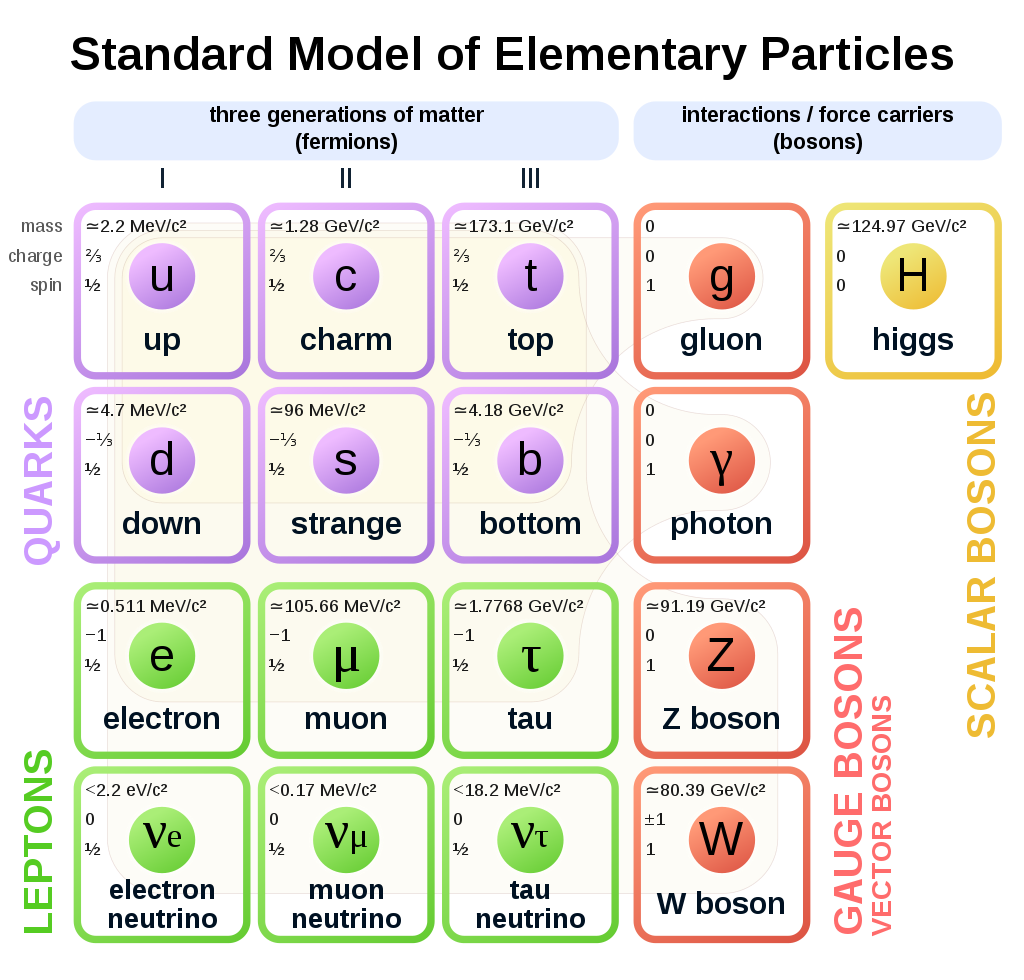
\includegraphics[scale=0.25]{Standard_Model.png}
		\caption{A figure showing the fundamental fermions and bosons of the SM \cite{StandardModelImage}.}
		\label{Fig:StandardModel1} 
	\end{figure}

	\subsubsection{Fermions}

	Due to Fermi-Dirac statistics, each fermion has a corresponding anti-particle: a particle with the same mass and spin but with opposite quantum numbers under charge-parity-time (CPT) conjugation. Fermions can be further subdivided into quarks and leptons by their interactions with the strong force: both contain three generations of of fundamental fermions with increasing mass, however quarks possess a colour charge whereas leptons do not. \par
	
	Colour in this sense does not refer to the typical description of colour, but a quantum number that parametrises these strong interactions with the value of either red ($r$), green ($g$), or blue ($b$) for particles and anti-red ($\bar{r}$), anti-green ($\bar{g}$) or anti-blue ($\bar{b}$) for anti-particles. The strong force binds particles with complementary colour charges together in order to create colourless states with no overall colour: 
	
	\begin{itemize}
		\item States with an equal mixture of red, green, and blue ($rgb$)
		\item States with an equal mixture of anti-red, anti-green, and anti-blue ($\bar{r}\bar{g}\bar{b}$)
		\item States with a colour-anticolour pair ($r\bar{r}$,$g\bar{g}$,$b\bar{b}$)
	\end{itemize}

	Gluons themselves possess a colour charge, and can be any combination of colour-anticolour pair that produces a net colour charge (i.e. excluding the previously addressed colourless states. This powerful binding by the strong force prevents the existence of individual quarks, causing quarks to be bound into colourless states called hadrons by the phenomenon of colour confinement. Hadrons consisting of three quarks/anti-quarks are called baryons/anti-baryons, and hadrons consisting of quark-antiquark pairs are called mesons. \par

	The three generations of quark are composed by doublets of one up-type quark and one down-type quark. These generations in order of increasing mass are:
	
	\begin{itemize}
		\item The first generation quarks, up ($u$) and down ($d$)
		\item The second generation quarks, charm ($c$) and strange ($s$)
		\item The third generation quarks, top ($t$) and bottom ($b$)
	\end{itemize}
	
	Each quark has an electric charge, $Q$, which is described relative to the electron charge. Up-type quarks ($u$, $c$, $t$) have a charge of $+\frac{2}{3}$, and down-type quarks have a charge of ($d$, $s$, $b$) have a charge of $-\frac{1}{3}$. In addition to charge and colour charge, the $u$ and $d$ quarks possess a quantum number named Isospin ($I$), and these quarks are assigned third component isospins ($I_{3}$) of $+\frac{1}{2}$ and $-\frac{1}{2}$ respectively. Table \ref{tab:SMQuarks1} summarises the properties of the SM quarks.

	% 04/03/21

	\begin{table} [h!]
		\begin{center}
			\begin{tabular}{ c|c|c|c|c }
				\hline \hline
				Generation & Quark Flavour & Mass [MeV] & $Q$ (e) & Colour Charge \rule{0pt}{2.6ex}\rule[-0.9ex]{0pt}{0pt}\\ 
				\hline \hline
				\multirow{2}{*}{1} & u & 2.2 & $+\frac{2}{3}$ & $r,g,b$ \rule{0pt}{2.6ex}\rule[-0.9ex]{0pt}{0pt}\\ 
								   & d & 4.7 & $-\frac{1}{3}$ & $r,g,b$ \rule{0pt}{2.6ex}\rule[-1.6ex]{0pt}{0pt}\\ 
				\hline
				\multirow{2}{*}{2} & c & 1.28$\times 10^{3}$ & $+\frac{2}{3}$ & $r,g,b$ \rule{0pt}{2.6ex}\rule[-0.9ex]{0pt}{0pt}\\ 
								   & s & 95 & $-\frac{1}{3}$ & $r,g,b$ \rule{0pt}{2.6ex}\rule[-1.6ex]{0pt}{0pt}\\
				\hline
				\multirow{2}{*}{3} & t & 173$\times 10^{3}$ & $+\frac{2}{3}$ & $r,g,b$ \rule{0pt}{2.6ex}\rule[-0.9ex]{0pt}{0pt}\\
				                   & b & 4.18$\times 10^{3}$ & $-\frac{1}{3}$ & $r,g,b$ \rule{0pt}{2.6ex}\rule[-1.6ex]{0pt}{0pt}\\
				\hline \hline

			\end{tabular}
			\caption{A table showing the mass, charge, and colour charge of the quark generations described by the SM \cite{Article:PDG2020}. \mbox{}\\}
			\label{tab:SMQuarks1}
			\begin{tabular}{ c|c|c|c|c }
				\hline \hline
				Generation & Lepton Flavour & Mass [MeV] & $Q$ (e) & Colour Charge \rule{0pt}{2.6ex}\rule[-0.9ex]{0pt}{0pt}\\
				\hline \hline
				\multirow{2}{*}{1} & $e$ & 0.511 & -1 & \multirow{2}{*}{---} \rule{0pt}{2.6ex}\rule[-0.9ex]{0pt}{0pt}\\
				                   & $\nu_{e}$ & $< 2\times10^{-3}$ & 0 & \rule{0pt}{2.6ex}\rule[-0.9ex]{0pt}{0pt}\\
				\hline
				\multirow{2}{*}{2} & $\mu$ & 106 & -1 & \multirow{2}{*}{---} \rule{0pt}{2.6ex}\rule[-0.9ex]{0pt}{0pt}\\
				                   & $\nu_{\mu}$ & $< 0.19$ & 0 & \rule{0pt}{2.6ex}\rule[-0.9ex]{0pt}{0pt}\\
				\hline
				\multirow{2}{*}{3} & $\tau$ & 1777 & -1 & \multirow{2}{*}{---} \rule{0pt}{2.6ex}\rule[-0.9ex]{0pt}{0pt}\\
				                   & $\nu_{\tau}$ & $ < 18.2$ & 0 & \rule{0pt}{2.6ex}\rule[-0.9ex]{0pt}{0pt}\\
				\hline \hline
			\end{tabular}
				\caption{A table showing the mass, charge, and colour charge of the leptons described by the SM \cite{Article:PDG2020}. \mbox{}\\} 
				\label{tab:SMLeptons1}
			\begin{tabular}{ c|c|c|c|c|c }
					\hline \hline
					Boson & Interaction & Mass [GeV] & $Q$ (e) & Colour Charge & Spin \rule{0pt}{2.6ex}\rule[-0.9ex]{0pt}{0pt}\\
					\hline \hline
					$\gamma$ & EM & 0 & 0 & --- & 1 \rule{0pt}{2.6ex}\rule[-0.9ex]{0pt}{0pt}\\
					\hline
					$W^{\pm}$ & Weak & 80.38 & $\pm 1$ & --- & 1 \rule{0pt}{2.6ex}\rule[-0.9ex]{0pt}{0pt}\\ \hline
					$Z$ & Weak & 91.19 & 0 & --- & 1 \rule{0pt}{2.6ex}\rule[-0.9ex]{0pt}{0pt}\\ \hline
					$g$ & Strong & 0 & 0 & 8 possible colour-anticolour pairs & 1 \rule{0pt}{2.6ex}\rule[-0.9ex]{0pt}{0pt}\\ \hline
					$h$ & Yukawa & 125.10 & 0 & --- & 0 \rule{0pt}{2.6ex}\rule[-0.9ex]{0pt}{0pt}\\ 
					\hline \hline
			\end{tabular}
					\caption{A table showing the respective interaction, mass, charge, colour charge, and spin of the bosons described by the SM \cite{Article:PDG2020}. \mbox{}\\}
					\label{tab:SMBosons1} 
		\end{center}
	\end{table}

	The three generations of leptons also exist in doublets, however these doublets consist of a negatively charged lepton and a corresponding neutrino with no electric charge. These three generations are:
	
	\begin{itemize}
		\item The first generation leptons, the electron ($e$) and electron neutrino ($\nu_{e}$)
		\item The second generation leptons, the muon ($\mu$) and muon neutrino ($\nu_{\mu}$)
		\item The third generation leptons, the tau ($\tau$) and tau neutrino ($\nu_{\tau}$)
	\end{itemize}

	Unlike the quarks, the leptons are have no colour charge and do not interact with the strong force whatsoever. While the masses of the charged leptons in each generation are well defined, neutrino masses have no intrinsic value within the SM. Experimental measurements of neutrino mixing, however, have determined an upper constraint for the neutrino masses of a small yet distinctly non-zero mass. Table \ref{tab:SMLeptons1} summarises the properties of the SM leptons. 

	\subsubsection{Bosons}
	
	The spin-1 gauge bosons\footnote{The "gauge" in "gauge bosons" arises from the gauge theories that describe the behaviour of the fundamental forces (see Section \ref{Section:GaugeTheory} and beyond).} of the SM mediate the interactions between particles under the fundamental forces. These bosons are:

	\begin{itemize}
		\item The photon ($\gamma$) which mediates electromagnetic interactions
		\item The $W^{+}$, $W^{-}$, and $Z$ bosons which mediate weak nuclear interactions
		\item The gluon ($g$) which mediates strong interactions
	\end{itemize}

	A spin-2 boson called the graviton has been proposed as a mediator of the gravitational force, however no experimental evidence of its existence has yet been observed. The ranges of each of the fundamental forces are limited by the Heisenberg uncertainty principle of $\Delta E \Delta t > \frac{\hbar}{2}$, as $\Delta E$ for each force is dependent upon the mass of the mediator boson. The more massive bosons of the weak interaction have a much shorter range than the massless photon, which allows electromagnetic interactions to occur over an infinite range. The proposed graviton would also allow an infinite range for the gravitational force, however this is not the case for the strong force due to the ability of the gluon to self-interact (see Section \ref{Section:QCD}). \par

	The final boson of the SM is the massive spin-0 Higgs boson, which does not mediate the interactions under one of the fundamental forces, but instead mediates interactions between massive particles and the Higgs field \cite{DiscoHiggsATLAS}\cite{DiscoHiggsCMS}. The mass of fermions, the gauge bosons, and the Higgs boson itself are all due to various interactions with the Higgs boson. Table \ref{tab:SMBosons1} summarises the properties of the SM bosons. 
	
	% 08/03/21

	\section{Standard Model Interactions}

	The equations of motion for this system are governed by the Principle of Least Action: The manner in which a system evolves between two states is described by the trajectory that minimises the action (S). For example, the motion of a free particle between two points would follow the path of a straight line, as this path requires the least possible energy and therefore minimises the action. The action is defined as:
	
	\begin{equation}
		S = \int \,d^{4}x \mathcal{L}[\phi(x^{\mu}),\partial_{\mu}\phi(x^{\mu})]
	\end{equation}

	where $\mathcal{L}[\phi(x^{\mu},\partial_{\mu}\phi(x^{\mu})]$ represents the Lagrangian density of the field $\phi(x^{\mu})$ and $x^{\mu}$ is the four-vector notation of $x$ such that\footnote{"Lagrangian density" and "$x^{\mu}$" will henceforth be written as "Lagrangian" and "x" respectively, so that the author may follow the Principle of Least Action while writing.}:
	
	\begin{equation}
		x^{\mu} = (t, x, y, z)
		\quad\mathrm{and}\quad
		x_{\mu} = (t, -x, -y, -z)
	\end{equation} 

	\begin{equation}
		\partial_{\mu} \equiv \frac{\partial}{\partial x^{\mu}}=(\frac{\partial}{\partial t}, \frac{\partial}{\partial x}, \frac{\partial}{\partial y}, \frac{\partial}{\partial z})
		\quad\mathrm{and}\quad
		\partial^{\mu} \equiv \frac{\partial}{\partial x_{\mu}}=(\frac{\partial}{\partial t}, -\frac{\partial}{\partial x}, -\frac{\partial}{\partial y}, -\frac{\partial}{\partial z})
	\end{equation}

	These principles allow the derivation of the Euler-Lagrange equation

	\begin{equation}
		\frac{\partial\mathcal{L}}{\partial\phi}=\partial_{\mu}\left(\frac{\partial\mathcal{L}}{\partial(\partial_{\mu}\phi)}\right)
	\end{equation}

	which is the basis for many of the classical mechanical equations of motion (e.g. Newton's Second Law). Just as the Lagrangian of a classical system would be used to obtain its equations of motion, the same is true of the SM, and the SM can be described by the Lagrangian formalism:

	\begin{equation}
		\mathcal{L}_{\mathrm{SM}} = \mathcal{L}_{\mathrm{EWK}} + \mathcal{L}_{\mathrm{QCD}} + \mathcal{L}_{\mathrm{Higgs}} + \mathcal{L}_{\mathrm{Yukawa}}
	\end{equation}

	\subsection{Gauge Theory} \label{Section:GaugeTheory}

	The concept of symmetry is fundamental to both the SM and physics as a whole, and is described by Noether's  theorem \cite{NoetherTheoremEnglish} which states that each symmetry of a system implies a conserved quantity. Perhaps the most simple example of this theorem is that of time symmetry: a system that experiences no change under a translation in time (i.e. the system is time symmetric), energy is conserved within that system. 
	
	In order to understand the SM, it is important to first understand the concept of a \textit{gauge} symmetry. Consider a complex scalar field with mass $m$ described by the Lagrangian:

	\begin{equation}
		\mathcal{L} = \partial^{\mu} \psi^{\dagger} \partial_{\mu} \psi - m^{2}\psi^{\dagger}\psi
	\end{equation}

	Under a rotation in the complex plane of angle $\alpha$ where

	\begin{equation}
		\psi(x) \rightarrow e^{i\alpha}\psi(x)  
		\quad\mathrm{and}\quad
		\psi^{\dagger}(x) \rightarrow e^{-i\alpha}\psi^{\dagger}(x)
	\end{equation}

	the lagrangian can be seen to be invariant as:

	\begin{equation}
		\begin{split}
		\mathcal{L} &= \partial^{\mu}  e^{-i\alpha} \psi^{\dagger} \partial_{\mu} e^{i\alpha} \psi  - m^{2}e^{-i\alpha} \psi^{\dagger} e^{i\alpha}\psi  \\
		&= (\partial^{\mu} \psi^{\dagger} \partial_{\mu} \psi - m^{2}\psi^{\dagger}\psi)(e^{-i\alpha}e^{i\alpha}) \\ 
		&= (\partial^{\mu} \psi^{\dagger} \partial_{\mu} \psi - m^{2}\psi^{\dagger}\psi)(e^{0}) \\
		&= \partial^{\mu} \psi^{\dagger} \partial_{\mu} \psi - m^{2}\psi^{\dagger}\psi \\
		\end{split}
	\end{equation}

	Therefore this lagrangian can be described as symmetric under global U(1) transformations: global, as $\alpha$ is invariant under transformation in $x$, and U(1) referring to the one-dimensional group of unitary transformations (which includes the previous transformation of the scalar field). Issues arise with this symmetry under a local transformation (i.e. where $\alpha$ depends on $x$). 
	% 17/02/21	

	Under this condition the mass term of the equation remains invariant, however the same is not true for the kinetic term as

	\begin{equation}
		\begin{split}
		\partial_{\mu}\psi &\rightarrow e^{i\alpha}\partial_{\mu}\psi+iq\partial_{\mu}\alpha e^{i\alpha}\psi \\
		&= e^{i\alpha}(\partial_{\mu}+i\partial_{\mu}\alpha)\psi \\
		\end{split}
	\end{equation}

	Restoring the local U(1) symmetry requires an update to the previous lagrangian: the introduction of a vector field, $A_{\mu}(x)$, that transforms as 
	
	\begin{equation}
		A_{\mu} \rightarrow A_{\mu} - \frac{1}{e} \partial_{\mu} \alpha
	\end{equation}

	This allows the definition of a new derivative such that

	\begin{equation}
		D_{\mu}\psi \rightarrow e^{i\alpha}D_{\mu}\psi
	\end{equation}

	allowing for invariance under a local U(1) transformation. This derivative is the covariant derivative, and it is defined as

	\begin{equation}
		D_{\mu} = \partial_{\mu} + ieA_{\mu}
	\end{equation}

	This can be checked by now observing the covariant derivative under a local U(1) transformation:

	\begin{equation}
		\begin{split}
			D_{\mu}\psi &\rightarrow (\partial_{\mu}+ie(A_{\mu}-\frac{1}{e}\partial_{\mu}\alpha))e^{i\alpha}\psi \\
			&= e^{i\alpha}\partial_{\mu}\psi + i\partial_{\mu}\alpha e^{i \alpha}\psi + iA_{\mu}e^{i\alpha}\psi - i\partial_{\mu}\alpha e^{i\alpha}\psi \\
			&= e^{i\alpha}(\partial_{\mu} + ieA_{\mu} + i\partial_{\mu}\alpha - i\partial_{\mu}\alpha)\psi \\
			&= e^{i\alpha}(\partial_{\mu}+ieA_{\mu})\psi \\
			&= e^{i\alpha}D_{\mu}\psi
		\end{split}
	\end{equation}

	With this change, the new Lagrangian under a local U(1) transformation becomes

	\begin{equation}
		\begin{split}
			\mathcal{L} &= e^{-i\alpha}D^{\mu}\psi^{\dagger}e^{i\alpha}D_{\mu}\psi - m^{2}e^{-i\alpha}\psi^{\dagger}e^{i\alpha}\psi \\
			&= (D^{\mu}\psi^{\dagger}D_{\mu}\psi - m^{2}\psi^{\dagger}\psi)(e^{-i\alpha}e^{i\alpha}) \\
			&= D^{\mu}\psi^{\dagger}D_{\mu}\psi - m^{2}\psi^{\dagger}\psi
		\end{split}
	\end{equation}

	% 25/02/21

	and the symmetry is restored. The new field $A_{\mu}$ which restores the local U(1) symmetry is referred to as the gauge field, and the modified Lagrangian as the gauge theory. \par

	% 02/03/21

	% 03/03/21 A lot of revisions to the above today.

	\subsection{Quantum Electrodynamics} \label{Section:QED}

	Quantum Electrodynamics (QED) is a gauge theory that covers the EM interactions between photons and fermions where $A_{\mu}$ represents the photon vector field and $\psi$ represents the charged fermion spinor fields. The Dirac Lagrangian describes interactions between these spinor fields

	\begin{equation}
		\mathcal{L}_{\mathrm{Dirac}} = \overline{\psi}(i\slashed{\partial}-m)\psi
	\end{equation}

	with $m$ representing the mass of the fermion, $\overline{\psi}=\psi^{\dagger}\gamma^{0}$, and $\slashed{\partial}=\gamma^{\mu}\partial_{\mu}$ where $\gamma^{\mu}$ is the four-vector notation of the Dirac gamma matrices:
	
	\begin{equation}
		\gamma^{\mu}=\begin{pmatrix}
			0 & \sigma^{\mu}  \\
			\overline{\sigma}^{\mu} & 0  \\
		\end{pmatrix}
	\end{equation}
	
	where $\sigma^{\mu}=(1,\sigma^{i})$, $\overline{\sigma}^{\mu}=(1,-\sigma^{i})$, and $\sigma^{i}$ represents the $2 \times 2$ Pauli matrices:

	\begin{equation}
		\sigma^{1}=\begin{pmatrix}
			0 & 1 \\
			1 & 0 \\
		\end{pmatrix},\quad\sigma^{2}=\begin{pmatrix}
			0 & -i \\
			i & 0 \\
		\end{pmatrix},\quad\sigma^{3}=\begin{pmatrix}
			1 & 0 \\
			0 & -1 \\
		\end{pmatrix}
	\end{equation}

	and under the Pauli-Dirac representation

	\begin{equation}
		\gamma^{0}=\begin{pmatrix}
			1 & 0 \\
			0 & -1 \\
		\end{pmatrix}
	\end{equation}

	such that

	\begin{equation}
		\gamma^{5} \equiv i\gamma^{0}\gamma^{1}\gamma^{2}\gamma^{3}=\begin{pmatrix}
			0 & 1 \\
			1 & 0 \\
		\end{pmatrix} 
	\end{equation}

	As in the previous example, this Lagrangian is invariant under a global U(1) transformation such that

	\begin{equation}
		\psi(x) \rightarrow e^{iq\alpha}\psi(x)  
		\quad\mathrm{and}\quad
		\overline{\psi}(x) \rightarrow e^{-iq\alpha}\overline{\psi}(x)
	\end{equation}

	however gauge invariance is lost under a global U(1) transformation. The symmetry can be restored with the introduction of the covariant derivative 
	
	\begin{equation}
		D_{\mu} = \partial_{\mu} - iqA_{\mu}
	\end{equation}

	and the photon vector field $A_{\mu}$ describing the interactions between fermions and photons which transforms as
	
	\begin{equation}
		A_{\mu} \rightarrow A_{\mu} + \partial_{\mu}\alpha(x)
	\end{equation}
	
	However, in order to form a complete QED Lagrangian it is also important to consider the kinematics of the $A_{\mu}$ field itself. This can be achieved with the introduction of the antisymmetric field strength tensor $F^{\mu\nu}$ which is defined as

	\begin{equation}
		\begin{split}
		F^{\mu\nu} &= \partial_{\mu}A_{\nu} - \partial{\nu}A_{\mu} \\
		&= -\frac{i}{q}[D^{\mu},D^{\nu}] \\
		\end{split}
	\end{equation}

	The introduction of this tensor results in a gauge invariant QED Lagrangian of the form

	\begin{equation}
		\mathcal{L}_{\mathrm{QED}}=\overline{\psi}(i\slashed{D}-m)\psi - \frac{1}{4}F_{\mu\nu}F^{\mu\nu}
	\end{equation}

	No other higher order terms (such as terms proportional to $A^{3}$ or proportional to $m^{2}A^{\mu}A_{\mu}$) are present in this Lagrangian, as their presence would remove the local gauge invariance. This prohibits the presence of both a mass term for the QED gauge boson (hence the massless nature of the photon), and any higher order terms for the photon field which prevents photon self interaction. 

	\subsection{Quantum Chromodynamics} \label{Section:QCD}

	Just as QED describes the interactions between photons and fermions, Quantum Chromodynamics (QCD) is a non-abelian gauge theory that describes the interactions between colour charged objects \cite{Article:QCDPrimer}. Unlike QED, this theory is not dependent on the unitary gauge group U(1) but the special unitary gauge group SU(3)$_{\mathrm{C}}$ where C denotes the colour charge of the fermions involved. The SU($n$) group is a subset of the U($n$) containing all unitary $n$ dimensional matrices with determinant 1. \par

	In this theory, quark fields possess one of the three colour charges ($r$, $g$, $b$) and anti-quark fields possess on of the three anti-colour charges ($\overline{r}$, $\overline{g}$, $\overline{b}$), represented by and transforming as fundamental colour triplets:
	
	\begin{equation}
		\psi_{f}(x) = \begin{pmatrix}
			\psi_{f}^{r}(x) \rule{0pt}{2.6ex}\rule[-0.9ex]{0pt}{0pt}\\
			\psi_{f}^{g}(x) \rule{0pt}{2.6ex}\rule[-0.9ex]{0pt}{0pt}\\
			\psi_{f}^{b}(x) \rule{0pt}{2.6ex}\rule[-0.9ex]{0pt}{0pt}\\
		\end{pmatrix}
	\end{equation}	
	
	where a single quark of flavour $f$ is represented as a superposition of the three fundamental colour states. The local transformation under the SU(3) group takes the form:
	
	\begin{equation}
		\psi(x) \rightarrow e^{i\alpha^{a}(x)T^{a}}\psi(x)
		\quad \mathrm{and} \quad
		\overline{\psi}(x) \rightarrow e^{-i\alpha^{a}(x)T^{a}}\overline{\psi}(x)
	\end{equation}

	where $\alpha^{a}(x)$ is a local phase shift, and $T^{a} = \frac{\lambda^{a}}{2}$ representing the generators of SU(3). In this case, $\lambda^{a}$ represents the 8 Gell-Mann matrices and $a$ is an index of the gluon colour charge. The Gell-Mann matrices take the form of
	
	\begin{equation}
		\begin{split}
			\lambda^{1}=&\begin{pmatrix}
				0 & 1 & 0 \\
				1 & 0 & 0 \\
				0 & 0 & 0 \\
			\end{pmatrix},\quad
			\lambda^{2}=\begin{pmatrix}
				0 & -i & 0 \\
				i & 0 & 0 \\
				0 & 0 & 0 \\
			\end{pmatrix},\quad
			\lambda^{3}=\begin{pmatrix}
				1 & 0 & 0 \\
				0 & -1 & 0 \\
				0 & 0 & 0 \\
			\end{pmatrix} \\
			\lambda^{4}=&\begin{pmatrix}
				0 & 0 & 1 \\
				0 & 0 & 0 \\
				1 & 0 & 0 \\
			\end{pmatrix},\quad
			\lambda^{5}=\begin{pmatrix}
				0 & 0 & -i \\
				0 & 0 & 0 \\
				i & 0 & 0 \\
			\end{pmatrix} \\
			\lambda^{6}=&\begin{pmatrix}
				0 & 0 & 0 \\
				0 & 0 & 1 \\
				0 & 1 & 0 \\
			\end{pmatrix},\quad
			\lambda^{7}=\begin{pmatrix}
				0 & 0 & 0 \\
				0 & 0 & -i \\
				0 & i & 0 \\
			\end{pmatrix},\quad
			\lambda^{8}=\frac{1}{\sqrt{3}}\begin{pmatrix}
				1 & 0 & 0 \\
				0 & 1 & 0 \\
				0 & 0 & -2 \\
			\end{pmatrix} \\
		\end{split}
	\end{equation}

	Gluons in this theory possess a combination of colour charged colour-anticolour pairs of which there are 8 possible combinations due to the interactions of the colour triplets with each of the 8 SU(3) generators. \par 

	Local invariance is preserved with the introduction of a new covariant derivative of the form

	\begin{equation}
		D_{\mu} = \partial_{\mu} + igT^{a}A_{\mu}^{a}
	\end{equation}

	with $g$ representing the strong coupling constant and $A_{\mu}^{a}$ the gluon field for colour charge $a$. This field transforms as

	\begin{equation}
		T^{a}A_{\mu}^{a} \rightarrow UA_{\mu}^{a}U^{\dagger}+\frac{i}{g}(\partial_{\mu}U)U^{\dagger}
	\end{equation}

	A crucial difference of QCD in comparison to QED is an additional term added to the field strength tensor: a term for the self interaction of gauge bosons. The QCD field strength tensor is defined as

	\begin{equation} \label{eq:GluonSelfInteract}
		\begin{split}
		F_{\mu\nu}^{a}&=\partial_{\mu}A_{\nu}^{a}-\partial_{\nu}A_{\mu}^{a}-gf^{abc}A_{\mu}^{b}A_{\nu}^{c} \\
		&=-\frac{i}{g}[D_{\mu},D_{\nu}]
		\end{split}
	\end{equation} 

	where $f^{abc}$ arises from the structure constants of SU(3) and the commutation relations of the generators of the group:

	\begin{equation}
		[T^{a},T^{b}] = if^{abc}T^{c}
	\end{equation}

	The self interaction term, $gf^{abc}A_{\mu}^{b}A_{\mu}^{c}$ in equation \ref{eq:GluonSelfInteract}, introduces one of the key differences between QCD and QED: the ability of multiple gluons to exchange colour between each other in the absence of fermions, and produce multi-gluon couplings. A second key difference is the asymptotic freedom exhibited by QCD. \par 
	
	In the case of QED interactions can occur at a potentially infinite range, with the strength of the coupling decreasing with distance. In the case of QCD, however, the coupling strength is strongest at large length scales. As two quarks bound by a virtual gluon are separated, the coupling strength also increases allowing for the creation of additional virtual gluons. \par
	
	Eventually, the virtual gluons would pass the energy threshold required to create quark-antiquark pairs, binding to the original quarks and preventing the creation of free colour-charged states. It is this characteristic of QCD that creates an upper limit for the range of the strong force despite the massless nature of the gluon. 

	The gauge invariant QCD Lagrangian takes the form

	\begin{equation}
		\mathcal{L}_{\mathrm{QCD}} = \sum_{f = 1}^{n_{f}}\overline{\psi}_{f}(i\slashed{D}-m_{f})\psi_{f}-\frac{1}{4}F_{\mu\nu}^{a}F_{a}^{\mu\nu}  
	\end{equation}

	with $m_{f}$ representing the quark mass of a quark with flavour $f$, and $n_{f}$ representing the total number of quark flavours. 

	\subsection{Electroweak Unification}

	The Glashow-Salam-Weinberg (GSW) model describes the behaviour of electroweak (EWK) interactions: interactions that occur when the electromagnetic and weak forces unify at the electroweak unification scale ($\approx$ 250 GeV). The GSW model is a non-abelian gauge theory constructed from the groups 
	
	\begin{equation}
		\mathrm{SU(2)}_{\mathrm{L}} \otimes \mathrm{U(1)}_{\mathrm{Y}}
	\end{equation}

	SU(2)$_{\mathrm{L}}$ contributes weak isospin ($T$) to the model, where L denotes the \textit{handedness} of the fermions involved. This property is related to a fermion's chirality\footnote{A particle can also have left- or right-handed \textit{helicity} depending on the direction of the particle's spin relative to its direction of motion, however (unlike chirality) helicity is not Lorentz invariant. The fermion shown in Figure \ref{Fig:Chirality} has right-handed helicity. A standard clock thrown face-forward at one's physics rival has left-handed helicity.}: an intrinsic quantum property that allows a particle to be classified as "left-handed" or "right-handed". Only left-handed fermions are affected by the gauge transformations of SU(2)$_{\mathrm{L}}$, which makes handedness a key concept of the GSW model. Figure \ref{Fig:Chirality} shows a graphical explanation of chirality. \par

	\begin{figure}[h!]
		\centering
		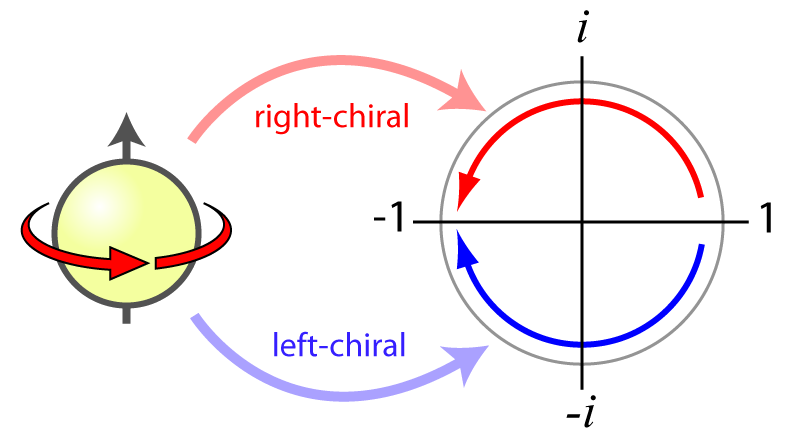
\includegraphics[scale=0.35]{complexrotation.png}
		\caption{A figure showing how left- and right-chiral fermions transform when rotated 360 degrees about their directions of motion. The circle on the right represents the complex phase of the particle's quantum state: as the particle is rotated, the value of the phase moves along the circle in a direction depending on the particle chirality \cite{ChiralityBlog}. }
		\label{Fig:Chirality} 
	\end{figure}

	U(1)$_{\mathrm{Y}}$ contributes weak hypercharge (Y) to the model. Both the weak hypercharge and weak isospin are related to the charge of the fermion via the equation

	\begin{equation}
		Q = T^{3} + \frac{Y}{2}
	\end{equation}

	where $T^{3}$ represents the third component of the weak isospin. 

	% 09/03/21

	In the GSW model left-handed fermions are described by separate weak isospin doublets for quarks and leptons of the form 

	\begin{align}
		Q_{L}&=\left\{\begin{pmatrix}
			u \\
			d \\
		\end{pmatrix}_{L},\begin{pmatrix}
			c \\
			s \\
		\end{pmatrix}_{L},\begin{pmatrix}
			t \\
			b \\
		\end{pmatrix}_{L}\right\} \\
		L_{L}&=\left\{\begin{pmatrix}
			\nu_{e} \\
			e \\
		\end{pmatrix}_{L},\begin{pmatrix}
			\nu_{\mu} \\
			\mu \\
		\end{pmatrix}_{L},\begin{pmatrix}
			\nu_{\tau} \\
			\tau \\
		\end{pmatrix}_{L}\right\}
	\end{align}

	where $Q_{L}$ and $L_{L}$ represent the states for quarks and leptons respectively. Right-handed fermions are described by separate weak isospin singlets for quarks and leptons of the form

	\begin{align}
		U_{R}&=\left\{u_{R},c_{R},t_{R}\right\} \\
		D_{R}&=\left\{d_{R},s_{R},b_{R}\right\} \\
		L_{R}&=\left\{e_{R},\mu_{R},\tau_{R}\right\}
	\end{align}

	where $U_{R}$, $D_{R}$, and $L_{R}$ represent the right handed up-type, down-type, and lepton states respectively. A notable exclusion from the right-handed singlets are the right-handed neutrinos which do not interact with the weak force. \par
	
	This is because while left-handed fermion doublets have $T=\frac{1}{2}$ with the upper and lower components of the doublet having $T^{3}=\pm\frac{1}{2}$ respectively, the right-handed singlets do not experience weak interactions and behave as SU(2)$_{\mathrm{L}}$ singlets. Resultantly, in the case of the right-handed neutrinos all quantum numbers relating to these states ($Q$, $T$, $T^{3}$, and $Y$) are 0 and therefore these states are not present (which follows experimental observation). \par

	These left-handed and right-handed states lead to a Dirac Lagrangian of SU(2)$_{\mathrm{L}} \otimes \mathrm{U(1)}_{\mathrm{Y}}$ that is comprised of a left-handed and right handed-component:
	
	\begin{equation}
		\mathcal{L}_{\mathrm{Dirac}} = \mathcal{L}_{\mathrm{Dirac},L} + \mathcal{L}_{\mathrm{Dirac},R}
	\end{equation}

	where

	\begin{align}
		\mathcal{L}_{\mathrm{Dirac},L}&=\sum_{g}\overline{Q}_{L}^{g}i\slashed{\partial}Q_{L}^{g}+\overline{L}_{L}^{g}i\slashed{\partial}L_{L}^{g} \\
		\mathcal{L}_{\mathrm{Dirac},R}&=\sum_{g}\overline{U}_{R}^{g}i\slashed{\partial}U_{R}^{g}+\overline{D}_{R}^{g}i\slashed{\partial}D_{R}^{g}+\overline{L}_{R}^{g}i\slashed{\partial}L_{R}^{g} 
	\end{align}

	The summation over the index $g$ represents the summation over all fermion generations, which will be assumed from this point onwards. The local transformations under SU(2)$_{\mathrm{L}}$ and U(1)$_{\mathrm{Y}}$ take the respective forms

	\begin{align}
		\psi(x) &\rightarrow e^{i\alpha^{a}(x)T^{a}}\psi(x) \\
		\psi(x) &\rightarrow e^{i\beta(x)g^{\prime}\frac{Y_{i}}{2}}\psi(x)
	\end{align}

	with $\alpha^{a}(x)$ and $\beta(x)$ representing complex phases, and $Y_{i}$ representing the hypercharge of fermion $i$. One covariant derivative must be defined for each transformation, taking the respective forms

	\begin{align}
		\textit{\textbf{D}}_{\mu} &= \partial_{\mu} + i\frac{g^{\prime}}{2}Y_{i}B_{\mu}+ig_{W}T^{a}W_{\mu}^{a} \\
		D_{\mu} &= \partial_{\mu} + i\frac{g^{\prime}}{2}Y_{i}B_{\mu} 	
	\end{align}

	where

	\begin{itemize}
		\item $B^{\mu}$ represents the hypercharge gauge field of U(1)$_{\mathrm{Y}}$ which couples to all fermions with coupling constant $g^{\prime}$
		\item $W_{\mu}^{a}$ represents the gauge fields of SU(2)$_{\mathrm{L}}$ which couple to all left-handed fermions with strength $g_{W}$
		\item $T^{a}=\frac{\sigma^{a}}{2}$ which represent the generators of SU(2)$_{\mathrm{L}}$ where $\sigma^{a}$ represents the $2 \times 2$ Pauli matrices as discussed in Section \ref{Section:QED}
	\end{itemize}

	The gauge fields $B^{\mu}$ and $W_{\mu}^{a}$ transform as

	\begin{align}
		B_{\mu} &\rightarrow U_{\mathrm{Y}}B_{\mu}U_{\mathrm{Y}}^{\dagger}-(ig^{\prime}\frac{Y_{i}}{2})^{-1}U_{\mathrm{Y}}^{\dagger}(\partial_{\mu}U_{\mathrm{Y}}) \\
		\textit{\textbf{W}}_{\mu} &\rightarrow U_{\mathrm{L}}\textit{\textbf{W}}_{\mu}U_{\mathrm{L}}^{\dagger}-(ig_{W})^{-1}(\partial_{\mu}U_{\mathrm{L}})U_{\mathrm{L}}^{\dagger}
	\end{align}

	where $\textit{\textbf{W}}_{\mu} = T^{a}W_{\mu}^{a}$. The field strength tensors for each field are defined as

	\begin{equation}
		\begin{split}
		B_{\mu\nu} &= -(i\frac{g^{\prime}}{2}Y_{i})^{-1}[D_{\mu},D_{\nu}] \\
		&= \partial_{\mu}B_{\nu} - \partial_{\nu}B_{\mu} \\
		\end{split}
	\end{equation}

	and

	\begin{equation} \label{eq:WSelfInteract}
		\begin{split}
			\textit{\textbf{W}}_{\mu\nu} &= -\frac{i}{g_{W}}[\textit{\textbf{D}}_{\mu},\textit{\textbf{D}}_{\nu}] \\
			&= T^{a}(\partial_{\mu}W_{\nu}^{a}-\partial_{\nu}W_{\mu}^{a}-g\epsilon^{abc}W_{\mu}^{b}W_{\nu}^{c}) \\
			&= T^{a}W_{\mu\nu}^{a} \\
		\end{split}
	\end{equation}

	where $\epsilon^{abc}$ is the Levi-Civita symbol which arises from the structure constants of SU(2)$_{\mathrm{L}}$ and the commutation relations of the generators of the group:

	\begin{equation}
		[\sigma^{a},\sigma^{b}]=i\epsilon^{abc}\sigma^{c}
	\end{equation}

	Just as the $gf^{abc}A_{\mu}^{b}A_{\nu}^{c}$ term in equation \ref{eq:GluonSelfInteract} allows for the self-interaction of gluons, the $g\epsilon^{abc}W_{\mu}^{b}W_{\nu}^{c}$ term in equation \ref{eq:WSelfInteract} allows for the self-interactions of the $W^{a}$ fields. \par

	The full electroweak Lagrangian including the field strength tensors to account for gauge field kinematics takes the form of

	\begin{equation}
		\begin{split}
		\mathcal{L}_{\mathrm{EWK}}=\overline{Q}_{L}i\slashed{D}Q_{L}+\overline{L}_{L}i\slashed{D}L_{L} &+ \overline{U}_{R}i\slashed{D}U_{R}+\overline{D}_{R}i\slashed{D}D_{R}+\overline{L}_{R}i\slashed{D}L_{R}\\
		&- \frac{1}{4}B_{\mu\nu}B^{\mu\nu}-\frac{1}{4}W_{\mu\nu}^{a}W^{\mu\nu,a}\\
		\end{split}
	\end{equation}

	Similarly to the previously derived $\mathcal{L}_{\mathrm{QED}}$ and $\mathcal{L}_{\mathrm{QCD}}$, there are no terms present in $\mathcal{L}_{\mathrm{EWK}}$ to account for the masses of fermions or gauge boson masses despite the experimental evidence to the contrary. This is due to the fact that these terms would violate the local SU(2)$_{\mathrm{L}} \otimes \mathrm{U(1)}_{\mathrm{L}}$ gauge invariance. In order to preserve this invariance, the source of the fermion and boson masses must be contributed by another source. 

	\subsection{Spontaneous Symmetry Breaking and the Higgs}

	% 10/03/21

	Just as each QFT of the SM is built upon a foundation of understanding the concept of gauge theory, the Higgs mechanism relies on an understanding of the concept of spontaneous symmetry breaking. A useful analogy for this concept is the behaviour of a ferromagnet. \par

	A ferromagnet held at a temperature above the Curie temperature effectively loses its magnetic properties: individual magnetic moments still exist within individual atoms, but the thermal agitation of the material causes such chaos amongst the alignment of these moments that the spacial average of the magnetic moment is zero. This creates a rotational symmetry for the system: rotating the ferromagnetic affects the spacial average of the magnetic moment in a similar manner that rotating a brick might, which is to say that it has no effect at all. \par
	
	However, if the temperature of the ferromagnet is reduced to a point \textit{below} the Curie temperature, the individual magnetic moments align in a direction parallel to each other and create an overall magnetic moment within the ferromagnet\footnote{The aforementioned brick is indifferent to the change in temperature as it is not ferromagnetic, and is thus a material that will not spontaneously break your symmetry or your heart.}. At this point the ferromagnet system now loses its rotational symmetry, causing this symmetry to be "spontaneously" broken as nothing in the Lagrangian of the system can account for this symmetry breaking effect. Figure \ref{Fig:SymmetryBreaking} shows a graphical description of this symmetry breaking. \par

	\begin{figure}[h]
		\centering
		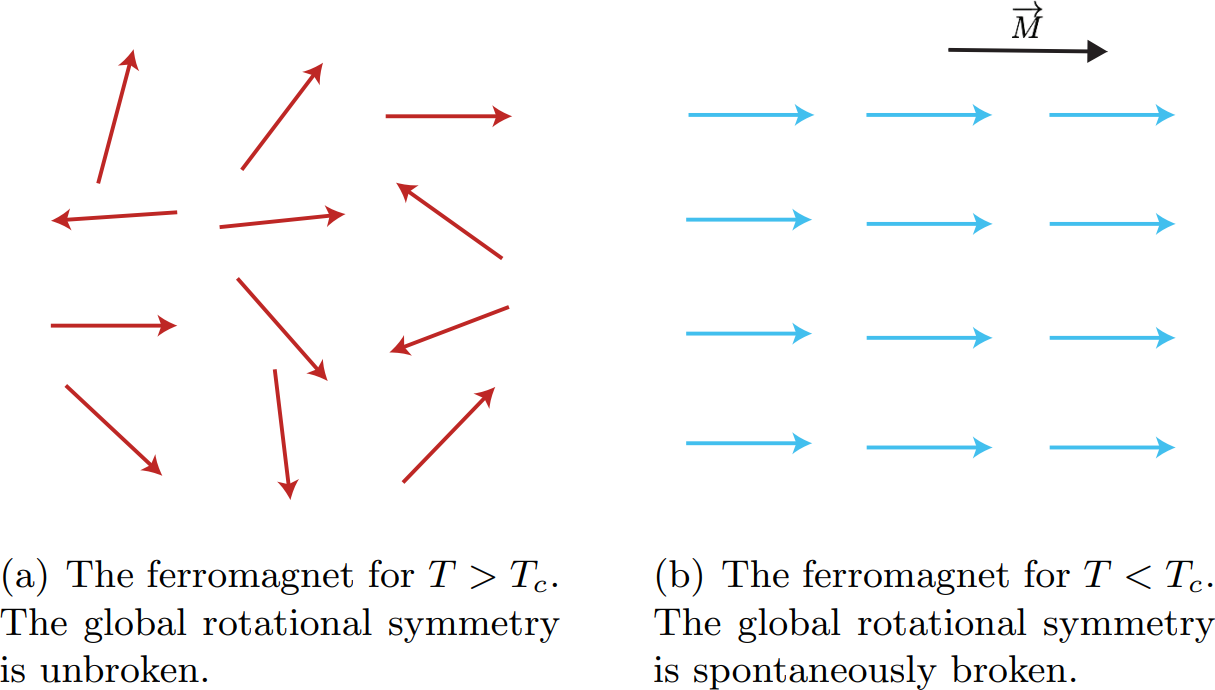
\includegraphics[scale=0.3]{Spontaneous_Symmetry_Breaking_HQ.png}
		\caption{A figure showing a two dimensional model of spontaneous global rotational symmetry breaking in a ferromagnet \cite{2012SpontaneousSB}.}
		\label{Fig:SymmetryBreaking} 
	\end{figure}

	While the description of this effect in field theory is far more quantitative than qualitative, the concept is the same and can be used as a basis for constructing a model that justifies the observed masses of the SM bosons. \par 

	\subsubsection{Global Spontaneous Gauge Symmetry Breaking}

	Consider the following scalar field theory:

	\begin{equation}
		\mathcal{L} = \frac{1}{2}(\partial_{\mu}\phi)^{2}-V(\phi)
	\end{equation}

	with

	\begin{equation} \label{eq:HiggsPotentialGlobal}
		V(\phi) = \frac{1}{2}\mu^{2}\phi^{2} + \frac{1}{4}\lambda\phi^{4}
	\end{equation}

	where $\lambda > 0$. Note that this Lagrangian has gauge invariance under transformations of the form $\phi \rightarrow -\phi$. There exists a value of $\phi$ such that the potential V($\phi$) is minimised, named the vacuum expectation value ($v$) of the field. This minimum of V($\phi$) can be determined by taking the derivative of V($\phi$) with respect to the field $\phi$ which takes the form of

	\begin{equation}
		\frac{dV}{d\phi}=(\mu^{2} + \lambda\phi^{2})\phi
	\end{equation}

	In the case where $\mu^{2}$ is real (i.e. $\mu^{2} > 0$) there is only a single solution where simply $v = 0$, named the vacuum field state configuration. This configuration has a unique minimum which preserves the gauge symmetry of the Lagrangian and leads to a conventional scalar particle mass term. \par

	The remaining solutions apply for the case where $\mu^{2} < 0$: in this configuration the vacuum field state configuration is instead a local maximum at $\phi = 0$ and two true degenerate minima are found at $\phi = \pm \sqrt{\frac{-\mu^{2}}{\lambda}}$. Figure \ref{Fig:HiggsPotential2D} shows the shapes of the potential for both $\mu^2$ cases.  

	\begin{figure}[ht]
		\begin{subfigure}{.48\textwidth}
			\centering
			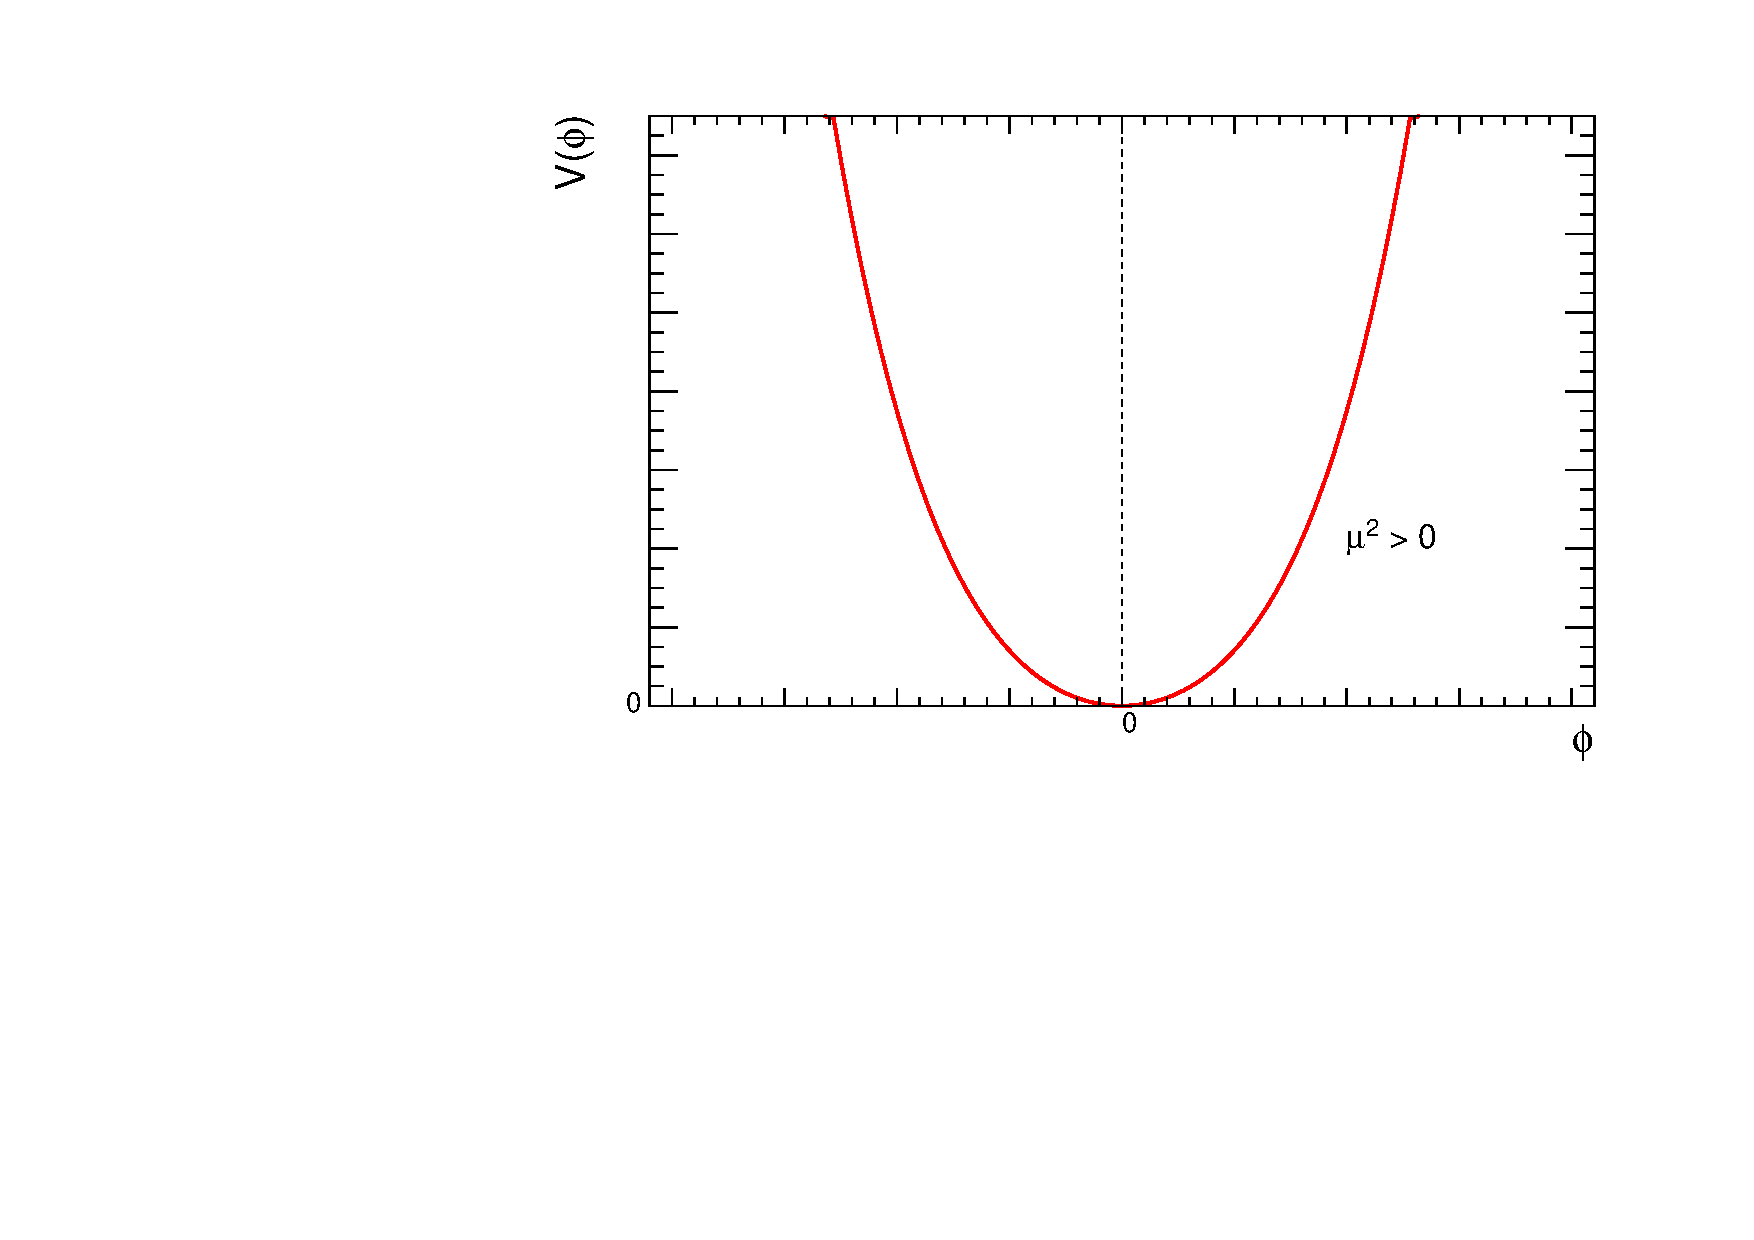
\includegraphics[scale=0.38]{HiggsPot_muEven.pdf}
			\label{Fig:HiggsPot_muEven}
		\end{subfigure}
		\begin{subfigure}{.48\textwidth}
			\centering
			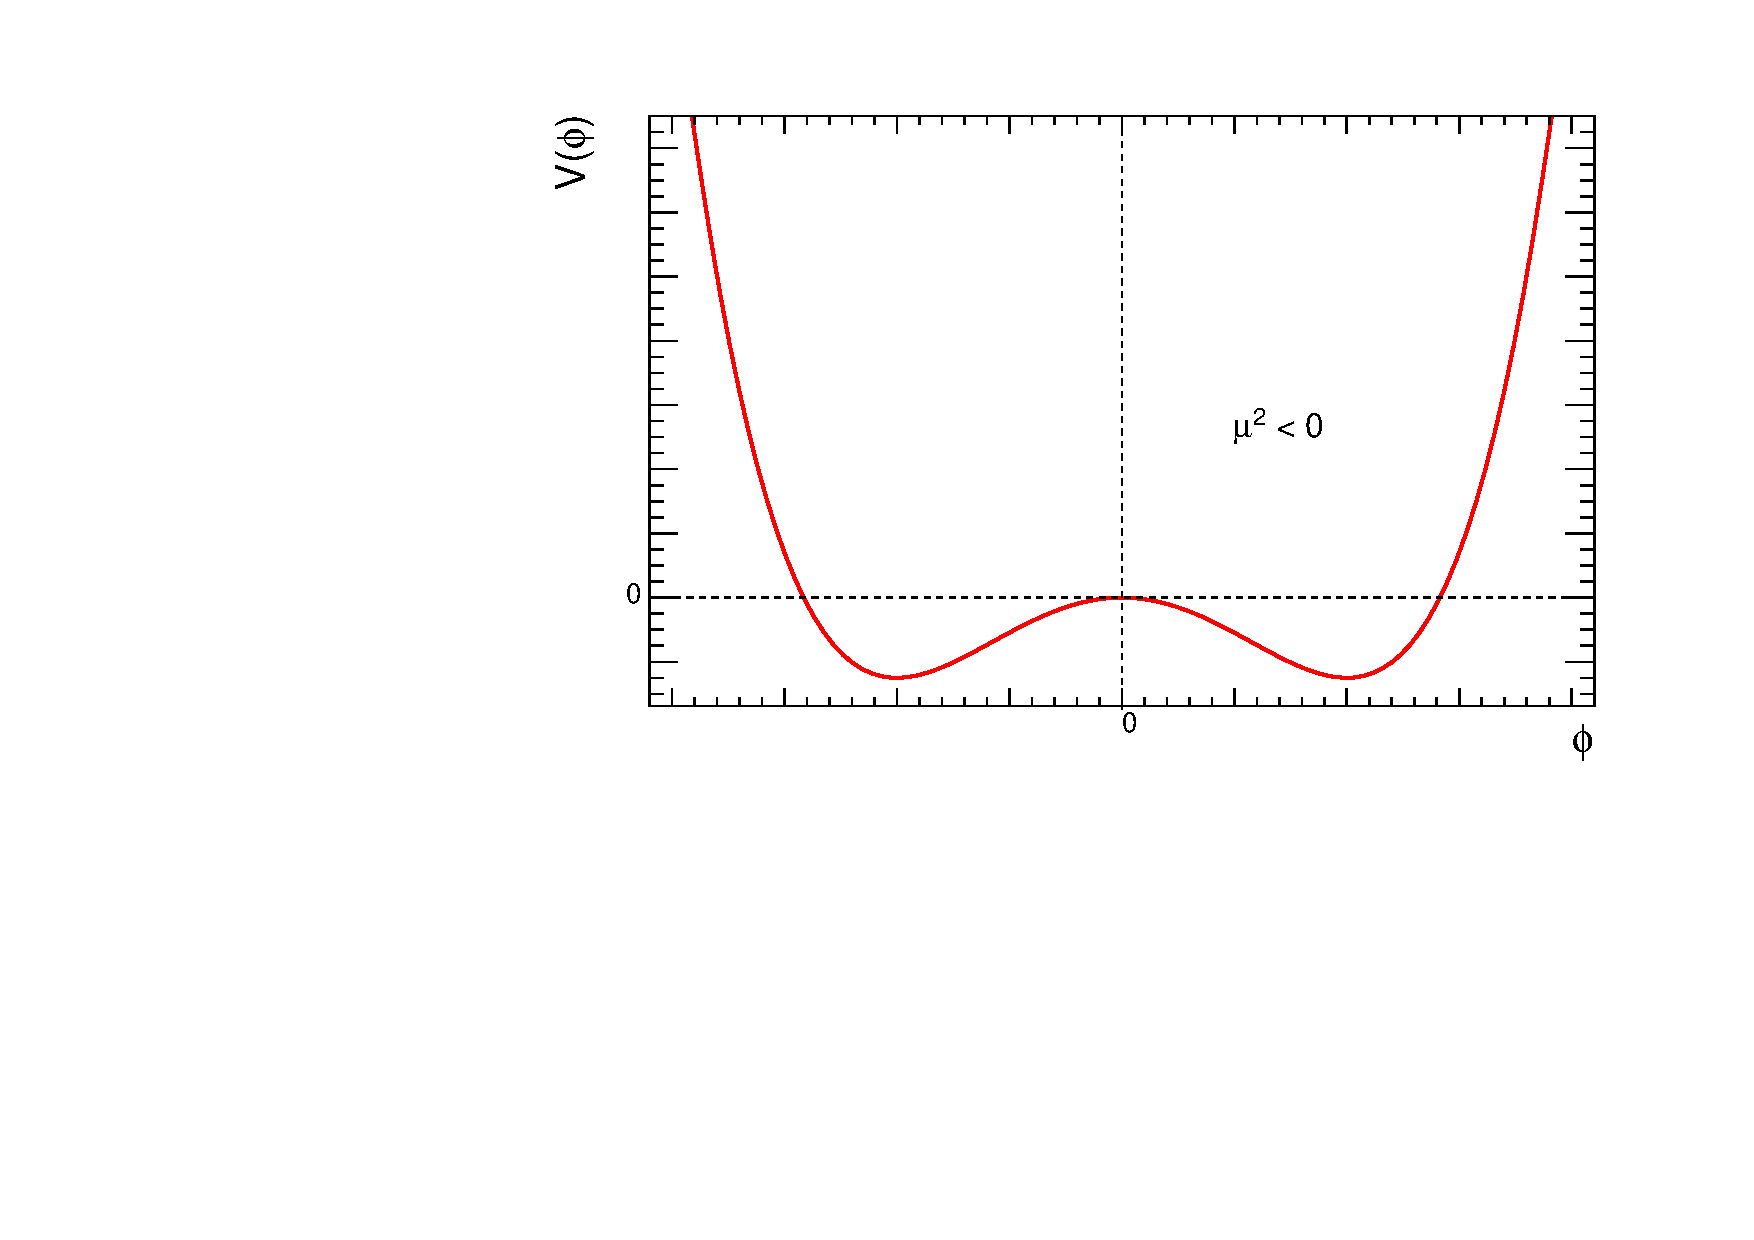
\includegraphics[scale=0.38]{HiggsPot_muOdd.pdf}
			\label{Fig:HiggsPot_muOdd}
		\end{subfigure}
		\caption{A figure showing the scalar field potential of Equation \ref{eq:HiggsPotentialGlobal} for the case of $\mu^2 > 0$ (left) and $\mu^2 < 0$ (right). The potential is weakest at a single point in the $\mu^{2} > 0$ case, and weakest at both of the minima for the $\mu^{2} < 0$ case \cite{AntonyFrayThesis}.}
		\label{Fig:HiggsPotential2D} 
	\end{figure}

	In the $\mu^2 < 0$ case where $v = \pm \sqrt{\frac{-\mu^{2}}{\lambda}}$, the scalar field $\phi$ can be redefined as

	\begin{equation}
		\phi(x) = v + \eta(x)
	\end{equation}

	where $\eta(x)$ represents a perturbation of the field about $v$. Using these definitions of $v$ and $\eta(x)$, the Lagrangian can now be rewritten as

	\begin{equation}
		\mathcal{L}(v + \eta) = \frac{1}{2}(\partial_{\mu}\eta)^{2}-\lambda v^{2}\eta^{2}-\lambda v\eta^{3}-\frac{1}{4}\lambda\eta^{4}+\frac{1}{4}\lambda v^{4}
	\end{equation}

	comparing this with the Klein-Gordon Lagrangian

	\begin{equation}
		\mathcal{L}_{\mathrm{KG}} = \frac{1}{2}\partial_{\mu}\phi\partial^{\mu}\phi-\frac{1}{2}m^{2}\phi^{2}
	\end{equation}

	it can be seen that the original mass term of the form

	\begin{equation}
		\begin{split}
		-\frac{1}{2}m^{2}\phi^{2} &= \frac{1}{2}(-|\mu^{2}|)\phi^{2} \\
		&= +\frac{1}{2}|\mu^{2}|\phi^{2}
		\end{split}
	\end{equation}

	has experienced a change in sign i.e.

	\begin{equation}
		+\frac{1}{2}|\mu^{2}|\phi^{2} \rightarrow -\lambda v^{2}\eta^{2}
	\end{equation}

	corresponding to a change from an imaginary configuration to a real configuration. 

	While the Lagrangian in this form retains its previous gauge symmetry under a transformation of the form $\phi \rightarrow -\phi$\footnote{In the form $\eta \rightarrow -2v-\eta$}, the vacuum field state configuration no longer satisfies this symmetry. The selection of either of the degenerate $v$ minima to expand about causes the original system's gauge symmetry to be spontaneously broken. 

	\subsubsection{The Higgs Mechanism}

	The mechanism that allows the introduction of gauge boson masses into the SM without violating $\mathrm{SU(2)}_{\mathrm{L}} \otimes \mathrm{U(1)}_{\mathrm{Y}}$ gauge invariance is provided by spontaneous symmetry breaking \cite{Brout-Englert}\cite{Higgs}. \par

	% 11/03/21

	Consider a complex doublet of scalar Higgs fields

	\begin{equation}
		\Phi=\begin{pmatrix}
			\phi^{+} \\
			\phi^{0} \\
		\end{pmatrix}=\begin{pmatrix}
			\frac{1}{\sqrt{2}}(\phi_{1}+i\phi_{2}) \\
			\frac{1}{\sqrt{2}}(\phi_{3}+i\phi_{4}) \\
		\end{pmatrix}
	\end{equation}

	where $\phi_{i}$ each represent real scalar fields. The Lagrangian of this system takes the form

	\begin{equation}
		\mathcal{L}_{\Phi} = T - V = (\textbf{D}_{\mu}\Phi)^{\dagger}(\textbf{D}^{\mu}\Phi)-\mu^{2}\Phi^{\dagger}\Phi+\lambda(\Phi^{\dagger}\Phi)^{2}
	\end{equation}

	where

	\begin{equation} \label{eq:HiggsPotential}
		V(\Phi^{\dagger}\Phi) = \mu^{2}\Phi^{\dagger}\Phi-\lambda(\Phi^{\dagger}\Phi)^{2}
	\end{equation}

	which is invariant under the SU(2)$_{\mathrm{L}}$ and U(1)$_{\mathrm{Y}}$ gauge transformations of the form 

	\begin{align}
		\phi(x) &\rightarrow e^{i\alpha^{a}(x)T^{a}}\phi(x) \\
		\phi(x) &\rightarrow e^{i\beta(x)g^{\prime}\frac{Y}{2}}\phi(x)
	\end{align}

	For this system, the covariant derivative is defined as

		\begin{equation}
			\textbf{D}_{\mu} = \partial_{\mu} + i\frac{g_{W}}{2}\textbf{W}_{\mu} + ig^{\prime}\frac{Y}{2}B_{\mu}
		\end{equation}

	\begin{figure}
		\begin{subfigure}{.48\textwidth}
			\centering
			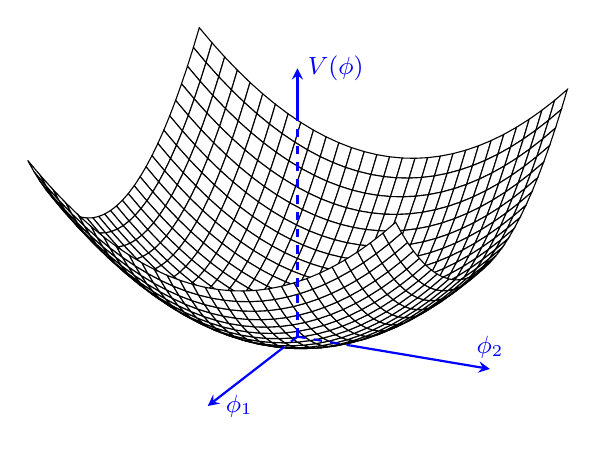
\begin{tikzpicture}
				\begin{axis}[
					hide axis,
					samples=30,
					domain=-0.9:0.9,
					y domain=-0.9:0.9,clip=false
				]
				\addplot3 [surf, shader=flat, draw=black, fill=white, z buffer=sort]
				({0.85*x},{0.85*y},{0.85*x^2+y^2});
				\draw[blue,thick,dashed] (axis cs:0,0,0) -- (axis cs:0.22,0,0);
				
				\draw[blue,thick,-stealth] (axis cs:0.22,0,0) -- (axis cs:0.8,0,0)
				node[above,font=\small]{$\phi_{2}$};
				\draw[blue,thick,dashed] (axis cs:0,0,0) -- (axis cs:0,-0.15,0);
				
				\draw[blue,thick,-stealth] (axis cs:0,-0.15,0) -- (axis cs:0,-0.8,0)
				node[right=1mm,font=\small]{$\phi_{1}$};
				\draw[blue,thick,dashed] (axis cs:0,0,0) -- (axis cs:0,0,1.55);
				\draw[blue,thick,-stealth] (axis cs:0,0,1.55) -- (axis cs:0,0,1.9)
				node[right,font=\small]{$V(\phi)$};
				\end{axis}
			\end{tikzpicture}
		\end{subfigure}
		\begin{subfigure}{.48\textwidth}
			\centering
				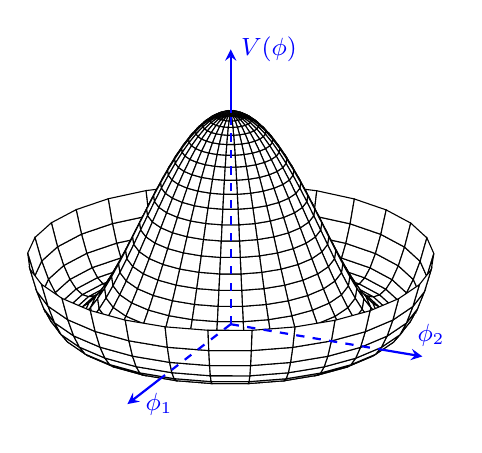
\begin{tikzpicture}
					\begin{axis}[
						hide axis,
						%axis lines=middle,
			%            axis on top,
			%            axis line style={blue,dashed,thick},
			%            ymin=-2,ymax=2,
			%            xmin=-2,xmax=2,
			%            zmin=-2,zmax=2,
						samples=30,
						domain=0:360,
						y domain=0:1.25,clip=false
					]
					\addplot3 [surf, shader=flat, draw=black, fill=white, z buffer=sort]
					({sin(x)*y}, {cos(x)*y}, {(y^2-1)^2});
					\draw[blue,thick,dashed] (axis cs:0,0,0) -- (axis cs:1,0,0);
					
					\draw[blue,thick,-stealth] (axis cs:1,0,0) -- (axis cs:1.3,0,0)
					node[above,font=\small]{~~$\phi_{2}$};
					\draw[blue,thick,dashed] (axis cs:0,0,0) -- (axis cs:0,-1,0);
					
					\draw[blue,thick,-stealth] (axis cs:0,-1,0) -- (axis cs:0,-1.5,0)
					node[right=1mm,font=\small]{$\phi_{1}$};
					\draw[blue,thick,dashed] (axis cs:0,0,0) -- (axis cs:0,0,1);
					
					\draw[blue,thick,-stealth] (axis cs:0,0,1) -- (axis cs:0,0,1.3)
					node[right,font=\small]{$V(\phi)$};
					\end{axis}
				\end{tikzpicture}
		\end{subfigure}
		\caption{A figure showing the scalar field potential of Equation \ref{eq:HiggsPotential} for the case of $\mu^2 > 0$ (left) and $\mu^2 < 0$ (right). The potential in the $\mu^2 > 0$ case is weakest at a single point, however it is weakest at an infinite number of points in the $\mu^2 < 0$ case. The right hand plot shows the famous "Mexican hat potential" of the Higgs, and the infinite number of points satisfying $v^{\prime}$ sit along the circumference of a circle around $V(\phi)$. }
		\label{Fig:HiggsPotential3D}
	\end{figure}

	Just as in the previous example, in the case where $\mu^{2} > 0$ there is a single solution for the vacuum expectation value where $v^{\prime} = 0$. In the case where $\mu^{2} < 0$, the potential is minimised when

	\begin{equation}
		|\Phi| = v^{\prime} = \sqrt{-\frac{\mu^{2}}{2\lambda}}
	\end{equation}

	which is a condition now satisfied by an infinite number of degenerate minima. This is visualised in Figure \ref{Fig:HiggsPotential3D} 

	$\Phi$ can now be rewritten in terms of the fields fluctuating about $v^{\prime}$. The form of this re-parametrisation is most simple in the U(1) gauge where 
	
	\begin{itemize}
		\item $v = 0$ for $\phi_{1}$, $\phi_{2}$, and $\phi_{4}$
		\item $\phi_{3}$ is set such that $\phi_{3}=h(x)+v^{\prime}$ where $h(x)$ is the Higgs field 
	\end{itemize}
		
	resulting in the form

	\begin{equation}
		\Phi = v = \frac{1}{\sqrt{2}}\begin{pmatrix}
			0 \\
			h(x)+v^{\prime}
		\end{pmatrix}
	\end{equation}

	Under this parametrisation, $\phi_{1}$, $\phi_{2}$, and $\phi_{4}$ represent massless Goldstone bosons. Goldstone's theorem states that for a Lagrangian that is invariant under a continuos symmetry, a massless scalar boson will be present for each generator of the symmetry that has been spontaneously broken \cite{GoldstoneTheorem}. In the case of the Higgs mechanism it is the symmetry of the SU(2)$_{\mathrm{L}}$ group with three generators that is spontaneously broken, hence the three Goldstone bosons. \par

	The $B_{\mu}$ and $\textbf{W}_{\mu}$ fields contained within $\textbf{D}_{\mu}$ can be redefined such that

	\begin{align}
		W^{+} &=\frac{1}{\sqrt{2}}(W^{1}_{\mu}+iW^{2}_{\mu}) \\
		W^{-} &=\frac{1}{\sqrt{2}}(W^{1}_{\mu}-iW^{2}_{\mu}) \\
		Z &=\cos\theta_{W}W^{3}_{\mu}-\sin\theta_{W}B_{\mu} \\
		A &=\sin\theta_{W}W^{3}_{\mu}+\cos\theta_{W}B_{\mu}
	\end{align}

	with 

	\begin{equation}
		\cos\theta_{W} = \frac{g_{W}}{\sqrt{g^{2}_{W}+g^{\prime 2}}}
	\end{equation}

	where $\theta_{W}$ is defined as the Weinberg angle. 

	Substituting all of the above into the original Lagrangian $\mathcal{L}_{\Phi}$ results in a Lagrangian of the form

	\begin{equation}
		\begin{split}
			\mathcal{L}_{\mathrm{Higgs}} &= \frac{1}{2}(\partial_{\mu}h)^{2} \\
			&+\frac{1}{2}\left(\frac{1}{2}g_{W}v^{\prime}\right)^{2}(W^{+}W^{-}+\text{complex conjugate})+\frac{1}{2}\left(\frac{\frac{1}{2}g_{W}v^{\prime}}{\cos\theta_{W}}\right)^{2}Z^{2} \\
			&+g_{W}\left(\frac{1}{2}g_{W}v^{\prime}\right)hW^{+}W^{-}+\frac{1}{4}v^{\prime}\frac{g^{2}_{W}}{\cos^{2}\theta_{W}}hZ^{2} \\
			&+\frac{1}{4}g^{2}_{W}h^{2}W^{+}W^{-} + \frac{1}{8}\frac{g^{2}_{W}}{\cos^{2}\theta_{W}}h^{2}Z^{2} \\
			&+\frac{1}{4}\lambda v^{\prime 4} - \lambda v^{\prime 2}h^{2} - \lambda v^{\prime}h^{3} - \frac{1}{4}\lambda h^{4}
		\end{split}
	\end{equation}

	where

	\begin{equation}
		V(\Phi^{\dagger}\Phi) = -\frac{1}{4}\lambda v^{\prime 4} + \lambda v^{\prime 2}h^{2} + \lambda v^{\prime}h^{3} + \frac{1}{4}\lambda h^{4}
	\end{equation}

	The system that once consisted of four massless scalar fields has now evolved into a system containing three massive gauge fields corresponding to the $W^{+}$, $W^{-}$, and $Z$ bosons, one massless gauge field corresponding to the photon, and one scalar Higgs field ($h$) while simultaneously preserving the SU(2)$_{\mathrm{L}}$ $\otimes$ U(1)$_{\mathrm{Y}}$ gauge invariance. \par
	
	In coupling with the Higgs field, the $W$ and $Z$ fields are said to have consumed the Goldstone bosons of the system. The masses of these bosons can be derived from the Higgs Lagrangian as

	\begin{equation}
		m_{W} = \frac{1}{2}g_{W}v^{\prime}
	\end{equation}
	\begin{equation}
		m_{Z} = \frac{1}{2}\frac{g_{W}v^{\prime}}{\cos\theta_{W}}
	\end{equation}

	and the mass of the Higgs boson itself is parametrised as 

	\begin{equation}
		m_{H} = \lambda v^{\prime 2}
	\end{equation}

	The additional terms of higher order in $h$ (i.e. $h^{3}$ and $h^{4}$) demonstrate the ability of the Higgs boson to self interact. 

	\subsubsection{Yukawa Mass Terms}

	The final missing pieces of the SM are the masses of the fermions, which are accounted for by the inclusion of a final Lagrangian describing Yukawa interactions between the Higgs and fermion fields. This Lagrangian takes the form

	\begin{equation}
		\mathcal{L}_{\mathrm{Yukawa}} = (-\mathcal{Y}_{L}\overline{L}^{i}_{L}\Phi_{i}L_{R}-\mathcal{Y}_{D}\overline{Q}^{i}_{L}\Phi_{i}D_{R}-\mathcal{Y}_{U}\epsilon_{ij}\overline{Q}^{i}_{L}\Phi^{*j}U_{R}) + \text{Hermitian conjugate}
	\end{equation}

	with $i$ and $j$ representing the weak isospin components of the SU(2)$_{\mathrm{L}}$ doublets. This Lagrangian implicitly sums over all three lepton and quark generations, with the coupling strength between the fermion and Higgs fields represented by the Yukawa couplings ($\mathcal{Y}$) which parametrise the fermion masses such that

	\begin{equation}
		m_{f} = \frac{1}{\sqrt{2}}\mathcal{Y}_{f}v^{\prime}
	\end{equation}

	Therefore under this formalism the couplings of the Higgs-fermion fields are dependent on the fermion-mass. An additional effect of this formalism is the massless nature of the neutrinos which is required by the SM.

	% 16/03/21

	\section{Collider Phenomenology}
	
	Fully describing the behaviour of \textit{pp} collisions requires a detailed understanding of the proton itself: the interaction that occurs during proton collisions does not take place between protons as a whole, but between the constituents of the protons. The proton is a baryon that exists as a configuration of three quarks: two up quarks and one down quark (\textit{uud}). It would be easy to assume that the proton simply shares its momentum equally between these three quarks and that any collision could be described with typical mechanical approaches, however this is simply not the case. \par

	The content of the proton is not static, but fluctuates: the three quarks that compose the proton (referred to as valence quarks in the context of particle structure) still possess individual colour charge when bound in a colourless bound state, and are able to interact with each other via the exchange of virtual gluons. Higher-order instances of these exchanges can even produce $q\overline{q}$ pairs within the proton referred to as sea-quarks. 

	\begin{figure}[ht]
		\centering
		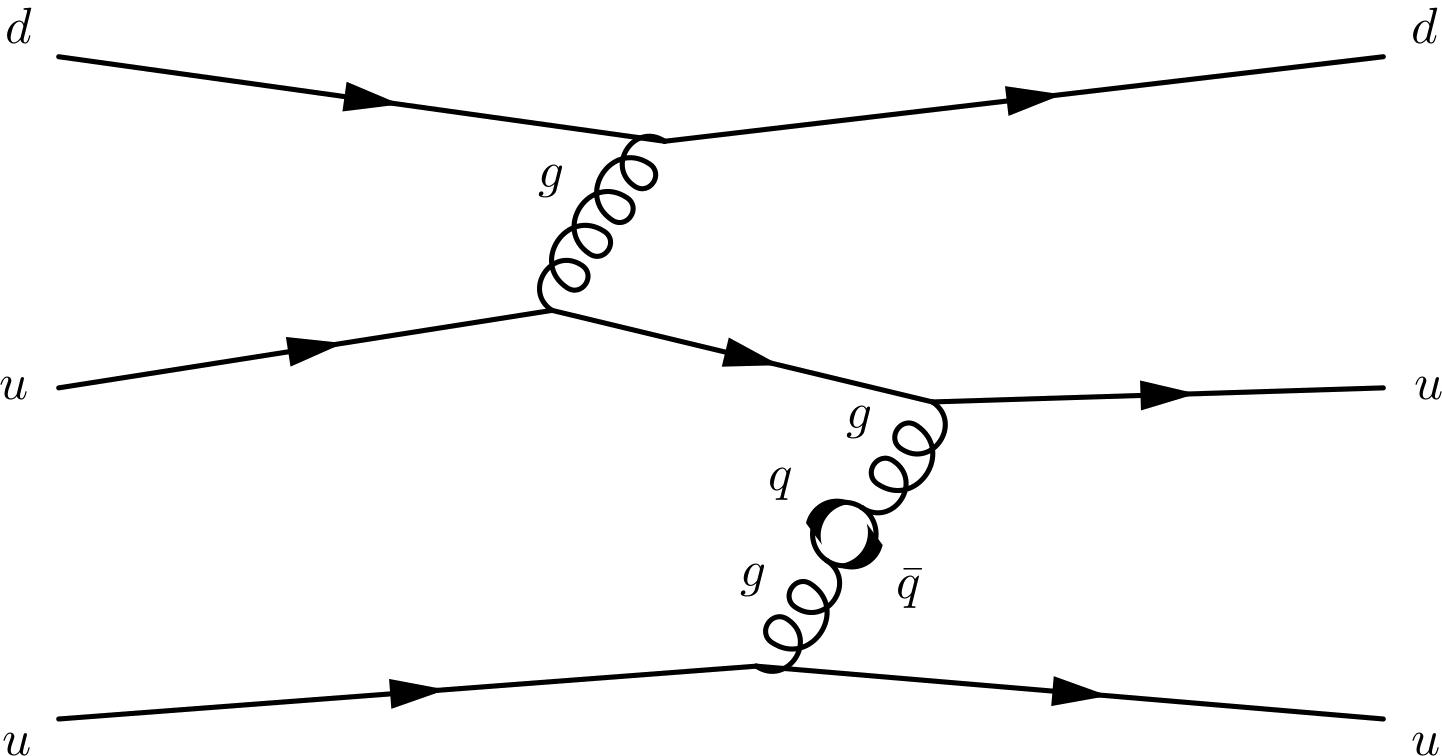
\includegraphics[scale=0.25]{Sea-quarks.png}
		\caption{A figure showing the exchange of gluons and $q\overline{q}$ pairs between valence quarks within the proton \cite{thomson_2013}.}
		\label{Fig:SeaQuarks} 
	\end{figure}

	Utilising \textit{pp} collision data to its fullest potential requires not just a profound understanding of the proton, but also an accurate description of the proton content and the manner in which it interacts. This is accomplished through the use of the Parton Model. \par

	\subsection{Parton Model}

	The Parton Model describes interactions involving the constituents of the proton, which are collectively referred to as \textit{partons}. The original model was proposed by Feynman to describe deep inelastic lepton-hadron scattering \cite{PartonModelFeynman}, which has been developed into the QCD improved parton model to describe high energy hadronic collisions \cite{PartonModelQCD}. In this model each hadron with four-momentum $P$ is described by its point-like parton constituents, with each parton carrying a fraction of the hadron's momentum labelled $x$. \par
	
	This momentum fraction can vary, with the momentum carried by each parton fluctuating as gluons are exchanged. The momentum of the partons for the hard scattering of an arbitrary interaction are expressed as Parton Distribution Functions (PDFs) $q(x, Q^{2})$, where $Q^{2}$ defines the energy scale for that particular interaction. Contributions from both gluons and quarks within the proton contribute to the PDF: contributions from gluons dominate the PDF at low $x$, while contributions from valence quarks dominate at high $x$. Due to this fact, \textit{pp} collisions at high energy can be treated as interactions purely between quarks and gluons. \par

	\subsection{Cross Section}

	Quark and gluon interactions can result in an immense number of final states, so it is crucial to know the probability of a particular process occurring when attempting a measurement. This probability is given by the cross-section ($\sigma$) of the process, measured in units of barns (1 b = $10^{-28}$ m$^{2}$). The cross-section of a particular interaction encodes the full production of a particular final state, which can be divided into two types of subprocesses: hard interactions and soft interactions. \par
	
	Typical particle collisions begin with a high energy hard scattering of partons, and are followed by lower energy soft interactions in the aftermath. Both hard and soft interactions are mediated by QCD, however hard processes can be described using perturbative techniques whereas the soft processes cannot. Factorisation Theorem \cite{HardProcessFactorization} is utilised where the typical approaches fail: under this theorem the cross section of a process can be described as
	
	\begin{equation}
		\sigma = \int dx_{1} \int dx_{2} \quad q_{1}(x_{1}, Q^{2})q_{2}(x_{2},Q^{2})\hat{\sigma}(x_{1},x_{2},Q^{2})
	\end{equation}

	where $\hat{\sigma}(x_{1},x_{2},Q^{2})$ represents the cross section of the hard scatter, and $q_{1}(x_{1},Q^{2})$ and $q_{2}(x_{2},Q^{2})$ represent the PDFs of the interacting partons which describe the soft interaction (which can be determined by experimental methods). \par

	The cross section is also important when determining the event rate of the events for a particular process, referred to as the luminosity (which is discussed in greater detail in Section \ref{Section:Luminosity}). 

	% 18/03/21 	

	\subsection{Signal Processes}
		
		The signal process for Z$\rightarrow$($\ell\ell$)+b or Z$\rightarrow$($\ell\ell$)+bb contain events where the Z boson decays to two muons or two electrons (Z$\rightarrow$($ee$) or Z$\rightarrow$($\mu\mu$)). This section describes the signal processes for Z$\rightarrow$($\mu\mu$) however the processes for Z$\rightarrow$($ee$) are similar, with the only difference being the decay products of the Z boson. \par
		
		The most common production of a Z boson which decays to two muons is through the Drell-Yan process \cite{Article:DrellYan} - a quark-antiquark pair from two colliding protons annihilate and produce two muons through the weak force mediated by a Z boson. However, in order to arrive at the final state either of the signal processes for this analysis (Z$\rightarrow$($\mu\mu$)+b or Z$\rightarrow$($\mu\mu$)+bb), an additional requirement must be met - the presence of one or two b-quarks. \par
		 
		The most common mechanism for this process to occur is for one of the annihilating quarks to radiate a gluon. The gluon then produces a pair of b-quarks (with one a standard b-quark, and the other an anti b-quark), meeting the requirements for the final state of the process. The Feynman diagram of this process can be seen in Figure \ref{Fig:SFigAnnihilationFeynman}. \par
		
		
		\begin{figure}[h!]
			\begin{subfigure}{.45\textwidth}
				\centering
				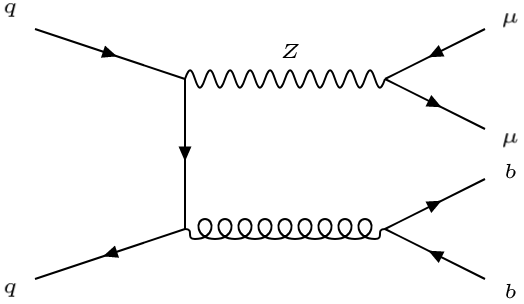
\includegraphics[scale=0.5]{Zbb_2.png}
				\caption{$q\overline{q}$ annihilation in conjunction with \newline the radiation of a gluon.}
				\label{Fig:SFigAnnihilationFeynman}
			\end{subfigure}
			\begin{subfigure}{.45\textwidth}
				\centering
				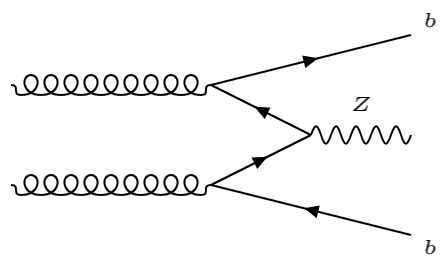
\includegraphics[scale=0.42]{Gluon_Pair.png}
				\caption{The final state produced by interactions \newline of a gluon pair.}
				\label{Fig:SFigGluonPairFeynman}
			\end{subfigure}
			\caption{A figure showing two possible mechanisms by which a Z$\rightarrow$($\mu\mu$)+bb final state can be achieved. }
			\label{Fig:FeynmanProcesses}
		\end{figure}
		
		\begin{comment}
		Another dominant process for this analysis is a single quark radiating both a Z boson and a gluon. Much like in the process of $q\overline{q}$ annihilation, the Z boson decays to two muons and the gluon produces a pair of b-quarks (with one being a standard b-quark, and the other its anti-particle). The Feynman diagram for this process can be seen in Figure \ref{Fig:SFigRadiationFeynman}. 
		\end{comment}
		
		
		Another dominant process for this production is a pair of gluons producing two quark-antiquark pairs. Each of the two gluons produces a bb pair, and interaction between the two pairs allows two of the quarks to annihilate and produce a Z boson (which later decays to two muons). The Feynman diagram for this process can be seen in Figure \ref{Fig:SFigGluonPairFeynman}. \par
		
		Finally, another process to be considered is that of the Compton process by which the interaction of a gluon with a single quark radiates a Z boson. It is this process that allows for the insight into the structure of the proton. At any one time, the content of a proton can be described by its PDF. \par
		
		The PDF of a given parton is a function of two variables: the fraction of the proton momentum carried by a parton ($x$), and the "scale" corresponding to the energy at which the parton is probed ($Q^{2}$). As the protons are collided inside the LHC beamline, the sea-quarks within the proton are able to interact with other partons such as valence quarks and gluons. For example in the case of Z$\rightarrow$($\mu\mu$)+b, the gluons and quarks interact via a hard process to produce a final state with one b-quark and a Z boson, which is subsequently detected by ATLAS. The cross section for this hard process can be written in the following form:
		
		\begin{comment}
		\begin{center}
			\begin{equation}
				\sigma (qg \rightarrow Zq) = \Sigma C_{i}^{P} (x,\alpha_{s}(Q^{2})) \otimes \tilde{f}_{i}(x,Q^{2},\alpha_{s}(Q^{2}))
			\end{equation}
		\end{center}
		With $C_{i}^{P}(x,\alpha_{s}(Q^{2}))$ as the perturbative calculable coefficient function, and $f_{i}(x,Q^{2},\alpha_{s}(Q^{2}))$ the probability to find a parton of type i carrying a fraction x of the proton momentum and $\tilde{f}_{i}(x,Q^{2},\alpha_{s}(Q^{2})) = xf_{i}(x,Q^{2},\alpha_{s}(Q^{2}))$ \cite{Article:PartonDistributions}. 
		\end{comment}
		
		\begin{center}
			\begin{equation}
			\frac{d\sigma}{dQ^{2}}=\sum_{i,j\in \{q,\overline{q},g\}}\int dx_{1}\int dx_{2}\; f_{i}(x_{1},Q^{2})f_{j}(x_{2},Q^{2})+f_{i}(x_{2},Q^{2})f_{j}(x_{2},Q^{2})\;\frac{d\hat{\sigma_{ij}}}{dQ^{2}}
			\end{equation}
		\end{center}
		
		With $\hat{\sigma}_{ij}$ as the cross section for (anti)-quarks and/or gluons, where $i$ and $j$ label the species of the colliding particle, and $f_{i}(x,Q^{2})$ the probability to find a particle of type $i$ carrying a fraction $x$ of the proton momentum\cite{Article:PartonDistributions}. When the process is detected, the momentum of the incident quarks can be calculated and used to perform a measurement of the proton PDF. PDFs are useful for calculating the cross sections of physical processes, and a measurement of Z$\rightarrow$($\mu\mu$)+b allows for a measurement of the proton PDF as well. The Feynman diagram for this process can be seen in Figure \ref{Fig:ZbbCompton}.
		
		\begin{figure}[h!]
			\centering
			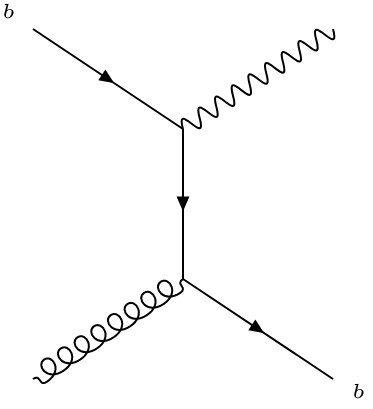
\includegraphics[scale=0.5]{Zbb_3.png}
			\caption{A figure showing the Feynman diagram for the Compton Process.}
			\label{Fig:ZbbCompton} 
		\end{figure}
			
		\subsection{Background Processes}
	
		As with the signal processes, the background process for Z$\rightarrow$($\ell\ell$)+b and Z$\rightarrow$($\ell\ell$)+bb are almost identical for both Z$\rightarrow$($ee$) and Z$\rightarrow$($\mu\mu$) with the only difference being the decay products of the Z boson. This section describes the processes for Z$\rightarrow$($\mu\mu$). \par
		
		The difficulty of Z$\rightarrow$($\mu\mu$)+bb analysis is in no small part due to the number of background processes that make a direct measurement difficult. In order to obtain a clear and accurate measurement of the signal process, there must be an equally clear understanding of the background processes such that any effect they have on a measurement of the signal process can be modelled and removed. \par
		
		The first and most common of these background processes is the top quark pair background. A pair of top quarks (specifically tt) are produced through one of many potential mechanisms, such as via a gluon interaction. Each top quark then undergoes a weak interaction to become a b quark, and produces a muon via a W boson and weak decay (as the overall charge of the process must be conserved). This results in the same final state as the Z$\rightarrow$($\mu\mu$)+bb signal process plus two additional neutrinos from the weak interaction of each top quark to a bottom quark. The Feynman diagram for this process can be seen in Figure \ref{Fig:SFigTtbarFeynman}. \par
		
		\begin{figure} [h!]
			\begin{subfigure}{.49\textwidth}
				\centering
				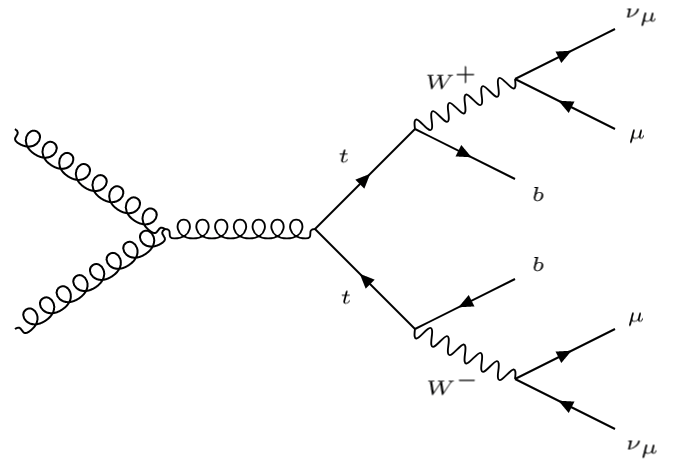
\includegraphics[scale=0.3]{Gluon_ttbar}
				\caption{The Top Quark Pair Production \newline background process.}
				\label{Fig:SFigTtbarFeynman}
			\end{subfigure}
			\begin{subfigure}{.49\textwidth}
				\centering
				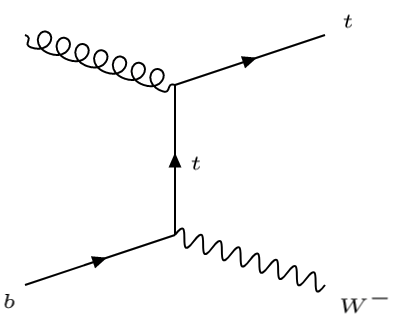
\includegraphics[scale=0.4]{Single_Quark}
				\caption{The Single Top background process.}
				\label{Fig:SFigWtFeynman}
			\end{subfigure}
			\caption{A figure showing the Feynman diagrams of Top Quark Pair Production and Single Top background production.}
			\label{Fig:FeynmanBackground1}
		\end{figure}
		
		\begin{comment}
		Similarly, instead of annihilating quarks exchanging a Z boson, a W boson can instead take its place. In this instance, instead of a top quark pair, a top quark and b-quark are produced. The top quark then decays to a second b-quark in the same manner as in the top quark pair background - the top quark changes flavour and the W boson decays to produce a muon and a neutrino. Unlike the top quark pair background, this single top background does not immediately appear to fulfil the final state of Z$\rightarrow$(\mu\mu)+bb. However, should this process occur in close proximity to another process in which a muon is produced, it could very easily be misidentified as a signal process. The Feynman diagram for this process can be seen in Figure \ref{Fig:SFigSTopFeynman}. 
		\end{comment}
		
		Another background process dependent on a charged current interaction is the single top background process. An incoming b-quark interacts with a gluon and experiences a weak interaction. A W boson is produced alongside a top quark, corresponding to the weak interaction of the b-quark. This results in the emission of only a single top quark, along with a W boson. This process can be seen in Figure \ref{Fig:SFigWtFeynman}. The final state is achieved by the weak interaction of first the top quark, which produces the necessary b-quark and an additional W boson, followed by the leptonic decay of two W bosons which produce a muon and a neutrino each. \par
		
		In addition to these background processes are the diboson background processes. In these interactions, annihilating quarks produce a combination of two bosons which produce	the required final state particles. The first of these processes is referred to as ZqqZll, in which both of the bosons produced are Z bosons. One Z boson decays to two leptons, and the second decays to two quarks. The most common source of this background in Z$\rightarrow$($\mu\mu$)+bb production is the case where one Z boson decays to two muons, and the other to two b-quarks. This	process can be seen in Figure \ref{Fig:SFigZqqZllFeynman}. \par
		
		The second of these diboson processes is referred to as WqqZll. This process is similar to the ZqqZll process, however in this instance only one of the produced bosons is a Z boson and the other is a W boson (as opposed to both being Z bosons). In this case, the W boson decays to two quarks, and	the Z boson to two leptons. The most common form that this background process takes in the Z$\rightarrow$($\mu\mu$)+bb analysis is the case where the W boson decays to a bottom quark and a charm quark, and the Z boson decays to produce two muons. This immediately fulfils the
		final state of the Z$\rightarrow$($\mu\mu$)+b processes, and can easily imitate the Z$\rightarrow$($\mu\mu$)+bb process if the charm quark is mistagged as a b-quark. These background processes (WqqZll and ZqqZll) are a small yet common background that is consistently present across the full energy range of the analysis. The Feynman diagram for these processes can be seen in Figure \ref{Fig:DibosonBackgroundFeynman}. \par
		
		
		\begin{figure}[h]
			\begin{subfigure}{.49\textwidth}
				\centering
				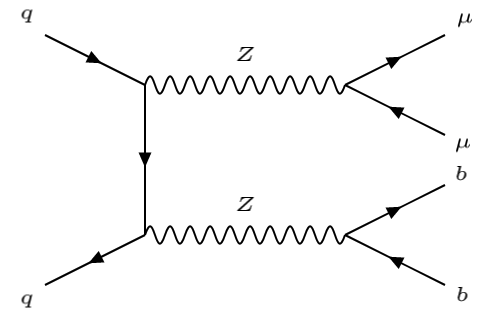
\includegraphics[scale=0.45]{ZqqZll}
				\caption{The ZqqZll background process.}
				\label{Fig:SFigZqqZllFeynman}
			\end{subfigure}
			\begin{subfigure}{.49\textwidth}
				\centering
				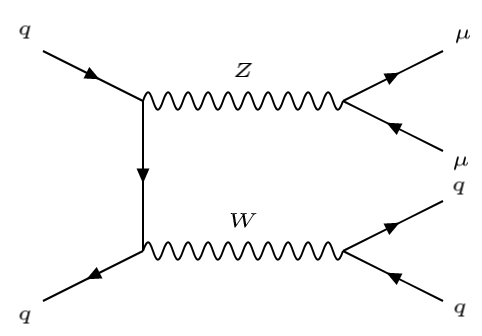
\includegraphics[scale=0.42]{WqqZll}
				\caption{The WqqZll background process.}
				\label{Fig:SFigWqqZllFeynman}
			\end{subfigure}
			\caption{A figure showing the Feynman diagrams for the WqqZll and ZqqZll background processes.}
			\label{Fig:DibosonBackgroundFeynman}
		\end{figure}  
		
		\begin{figure}[h!]
			\centering
			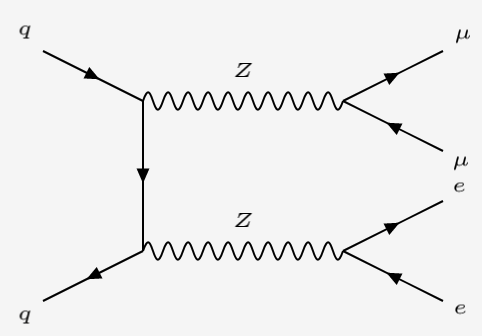
\includegraphics[scale=0.45]{ZZ4l}
			\caption{The ZZ4l background process.}
			\label{Fig:ZZ4lFeynman}
		\end{figure}
		
		
		In addition to the WqqZll and ZqqZll backgrounds mentioned above, there is an additional background process named ZZ4l which corresponds to an event where the two produced Z bosons decay into four leptons. The Feynman diagram for this process can be seen in Figure \ref{Fig:ZZ4lFeynman}. This background process occurs when one of the Z bosons produces two muons, and the other two electrons. Electrons produce jets along with
		electromagnetic showers within the electromagnetic calorimeters in ATLAS (see section 3.2.3), and a background process is found where this reconstructed jet is mistagged as a b-jet. \par
		
	\newpage

	\chapter{Experimental Setup}

		The source of all experimental data within this thesis is the ATLAS experiment at the Large Hadron Collider (LHC). The following chapters will provide an introduction to both the LHC and the ATLAS experiment with a primary focus on the subsystems of the ATLAS detector most relevant to this analysis. The data used in this thesis was collected during the second run of data collection by the LHC (appropriately named Run 2), which concluded in December of 2018. The third run of data collection will begin in 2021. 

		\section{The Large Hadron Collider}

		100 meters beneath the site of the Conseil Européen pour la Recherche Nucléaire (CERN) at the French-Swiss border near Geneva, Switzerland lies the LHC. At approximately 27 kilometres in circumference, the LHC accelerates beams of protons to the highest energies in the world 
		reaching speeds greater than 99.9\% the speed of light \cite{LHCDesignV1, LHCDesignV2, LHCDesignV3}. 

		\subsection{Acceleration at the LHC}

		Beginning with it's initial flagship accelerator, CERN has constantly upgraded its accelerators and included the work of previous experiments in each new effort to collect even greater amounts of particle collision data. The full acceleration of the particle beams within the LHC is not reliant on a single static machine but a combined effort from multiple component accelerators, each of which further accelerates beams of particles to higher and higher energies prior to collision. Each particle accelerated by the LHC experiences not just a chain of particle accelerators, but a timeline of CERN's remarkable history.   
		
		This chain of accelerators begins with an ordinary container of hydrogen: atoms of hydrogen are extracted from the canister and subjected to an ionising electric field, stripping the hydrogen atoms of their electrons and leaving only the protons remaining. This ionised hydrogen gas is then immediately fed into the Linear Accelerator 2 (LINAC2), which accelerates the protons up to an energy of 50 MeV. LINAC2 has been in operation since 1978 after replacing the original Linear Accelerator 1 (LINAC1), and will itself be replaced by the Linear Accelerator 4 (LINAC4) in Run 3 to further upgrade the LHC \cite{LINAC4}. \par 
		
		Following their linear acceleration through LINAC2, the protons then enter the first of the four circular accelerators within the LHC acceleration chain: the Proton Synchrotron Booster (PSB). The PSB accelerates the protons to an energy of 1.4 GeV, before injecting them into the Proton Synchrotron (PS) which increases the energy of the protons to 25 GeV. The PS first accelerated protons on 24 November 1959, serving as CERN's first synchrotron. While the PS has been heavily modified from its original state, it still serves as a key piece of LHC operations over 60 years later. \par

		From the PS, the protons are then injected into the even more powerful Super Proton Synchrotron (SPS): far larger than the 688 m circumference of the PS, the SPS has a circumference of 7 km and almost 5 times as many electromagnets, capable of accelerating the protons to an energy of 450 GeV. The SPS originally operated as the principle collider of CERN's particle physics program when it came online in 1976 and was crucial in several key experiments in CERN's history, such as the Nobel-prize-winning discovery of the W and Z bosons in 1983 when the SPS ran as a proton-antiproton collider \cite{WBosonDiscovery, ZBosonDiscovery}. 

		The final step in the accelerator chain is the LHC itself, however the method of accelerating within the LHC differs slightly from the techniques of the previous circular accelerators. The protons from the SPS are injected to the LHC at two points instead of one in order to create two separate proton beams which circulate in opposite directions. These two distinct beams are each accelerated up to an energy of 6.5 TeV, allowing for a centre-of-mass energy of $\sqrt{s}$ = 13 TeV during Run 2. The full chain of LHC accelerators can be seen in Figure \ref{Fig:CERNRings}. \par

		\begin{figure}
			\centering
			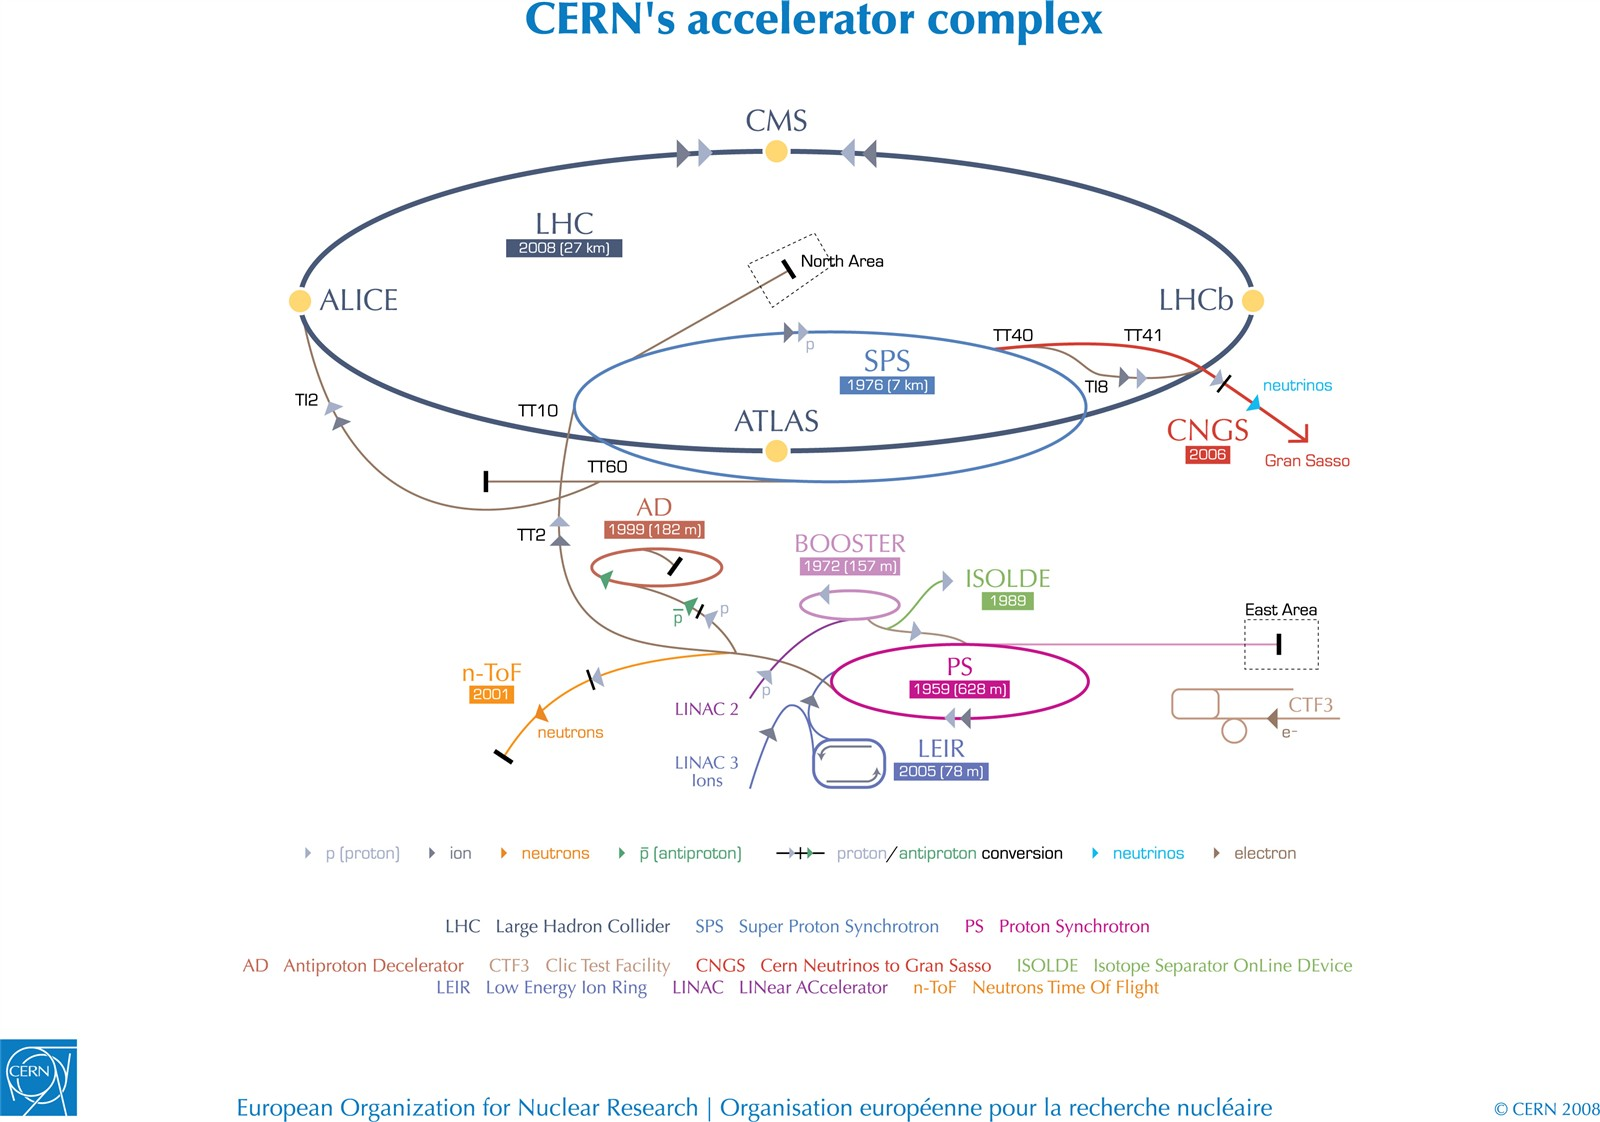
\includegraphics[scale=0.5]{LHC_Rings}
			\caption{A figure showing the arrangement and relative sizes of the accelerators within the LHC acceleration chain \cite{Article:CernComplex}.}
			\label{Fig:CERNRings}
		\end{figure}

		% End of rewrite to detector chapter 25/01/21

		Achieving the acceleration required to achieve these energies is no easy task. The tunnels in which the LHC resides were originally constructed for the Large Electron-Positron (LEP) collider \cite{LEPHistory, LEPDesign1, LEPDesign2, LEPDesign3}, a particle-antiparticle collider capable of accelerating two beams in opposite directions with the same magnetic field (due to the opposite charge between a charged particle and its respective antiparticle). The same method cannot be applied in the case of proton-proton collisions as the charge of each beam will be the same. Instead, the LHC uses its single magnet system to produced a pair of coupled magnetic fields which have an opposing polarity. \par

		The LHC does not, however, accelerate the particle beams at every point along its circumference. The LHC is composed of 8 octants, in which the LHC ring is actually a straight line. The curvature of the particle beams occurs at the boundaries of each octant, where 1232 powerful dipole magnets (each 15 metres long and with a weight of 35 tonnes) create a magnetic field of 8.3 T which bends the beams towards the centre of the LHC ring. These dipoles work in conjunction with 392 quadrupoles: magnets with alternating poles in a symmetrical layout that help focus the beam \cite{LHCMagnets}. In order to remain superconducting, these magnet are cooled with super-fluid Helium which allows the magnets to operate at 1.4 K. \par

		The straight sections of the LHC within each of the octants are referred to as "Points", and are numbered according to their position around the LHC ring. Each of these points can be seen in Figure \ref{Fig:CERNOctants}. Point 1, Point 2, Point 5, and Point 8 contain each of the interaction points (IPs) where the particle beams cross and interactions occur. Four large particle detectors of varying design are constructed at each of these IPs in order to observe the collisions that occur where the particle beams collide: two large general-purpose experiments ATLAS \cite{ATLAS_Collab} and CMS \cite{CMSCollab} at Point 1 and Point 5, the ALICE \cite{ALICECollab} experiment at Point 2 primarily examining heavy-ion collisions, and the LHCb \cite{LHCCollab} experiment at Point 8 primarily exploring flavour physics and CP-violation through bottom and charm quarks. \par

		\begin{figure}
			\centering
			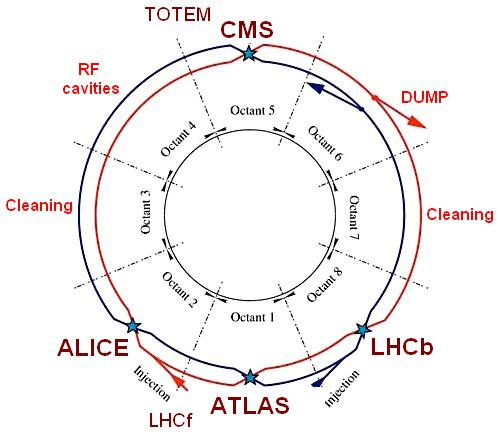
\includegraphics[scale=0.5]{LHC_Octants}
			\caption{A figure showing the arrangement of the LHC octants or "Points" \cite{Evans_2008}.}
			\label{Fig:CERNOctants}
		\end{figure}

		Point 3 and Point 7 contain the beam cleaning and collimation systems, essential systems that protect the components of the LHC. As proton beams travel around the LHC ring, they do not exist as a single some protons are unavoidably lost from the focussed central beam core and diffuse into a "beam halo", the fraction of the beam that will physically collide with the components of the LHC. These collisions from the beam halo can damage these components: for example, collisions with the LHC's superconducting magnets could cause a rise in temperature forcing the magnets out of a superconducting state (this is known as a magnet "quench") \cite{LHCCollimation1}. The collimator systems restrict the potential aperture of the beam, deliberately causing collisions with the beam halo to occur safely in the collimators (instead of in the LHC's more delicate subsystems) \cite{LHCCollimation2}. \par 

		The beam dump is located at Point 6, and is another important subsystem for the efficiency and safety of the LHC. When the particle beam within the LHC has served its purpose, the beam (or the remnants of it) needs to be safely removed from the LHC ring. The beam may also be dumped in the event of instability observed by the LHC or one of the detectors observing each of the IPs, or in the event of issues with one of the detectors. In the event that the beam needs to be dumped for any of these reasons, the LHC employs the use of kicker magnets that rapidly and safely diver the beam out of the LHC ring and into dump blocks: cylinders of graphite encased in concrete that can absorb the full energy of the beam without melting \cite{LHCDesignV2}. \par 
		
		The actual acceleration of the particle beam within the LHC occurs at the superconducting radio-frequency (RF) cavities located at Point 4. The LHC employs 8 RF cavities per beam, which use an alternating electric field to accelerate the beam through the cavity. By increasing the frequency of these oscillations, the particle beam can gradually increase to its maximum energy. Much like the dipole and quadrapole magnets used within the LHC, the RF cavities also operate at an extremely low temperature (4.5 K). The accelerating field provided by the RF cavities is 5 MV/m at 400MHz \cite{LHCRF}. Accelerating particles using the alternating electric field of the RF cavities causes the particle beam not to be a single continuous beam, but to instead be divided into \textit{bunches}.
		
		\subsection{Beam Structure}
		
		% 27/01/21

		When the particle beam passes through the RF cavities, some of the particles synchronize exactly with the RF frequency (these particles are aptly named "synchronous particles"). Particles that do not exactly synchronize with this frequency instead become clustered around the synchronous particle, and this travelling group of synchronized particles is referred to as a bunch. In order to allow for the necessary time for its subsystems to function correctly, the LHC beam is not a continuous stream of bunches but a combination of bunches and "missing" bunches (deliberate absences of bunches used primarily for timing). \par

		The nominal LHC beam consists of 2808 bunches, each consisting of $1.15 \times 10^{11}$ protons \cite{LHCDesignV1,LHCDesignV3}. The PS supplies particles to the SPS and LHC in the form of 72-bunch PS trains, with each bunch arriving 25 ns apart \cite{LHCBeam}. When these bunches are accelerated by the SPS and enter into the LHC, they are arranged into the form of 3, 3, and then 4 PS trains. The very last PS train in the very last SPS batch is deliberately suppressed to allow time for the LHC extraction kicker magnets (required in the event of a beam dump) to rise. This bunch structure can be observed in Figure \ref{Fig:LHCBunches}. 

		\begin{figure}
			\centering
			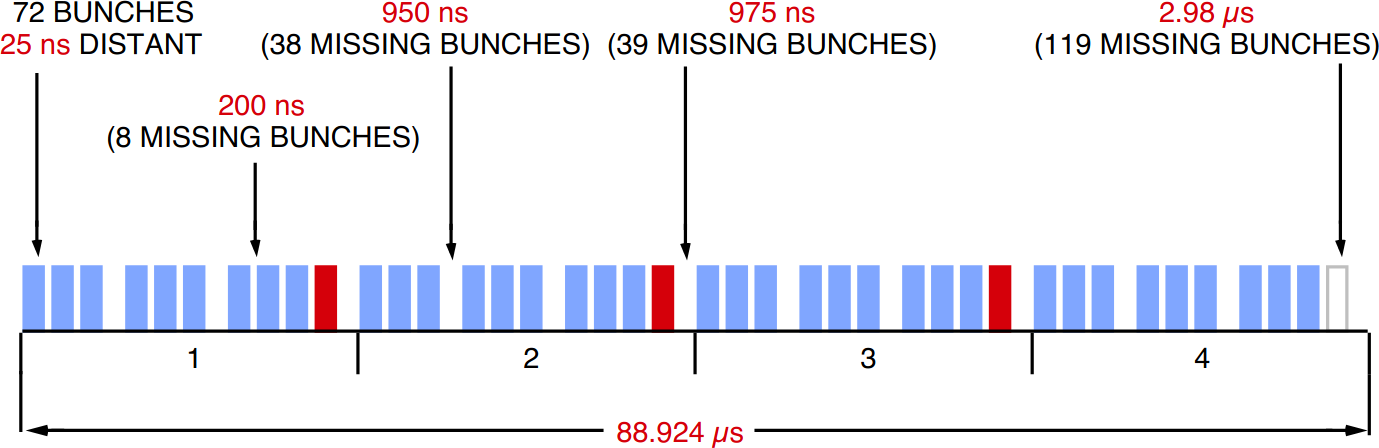
\includegraphics[scale=0.3]{LHC_Beam_Structure}
			\caption{A figure showing the arrangement of the PS trains within the final SPS batch injected into the LHC \cite{LHCBunches}.}
			\label{Fig:LHCBunches}
		\end{figure}

		% 28/01/21

		\subsection{Luminosity} \label{Section:Luminosity}

		In order to evaluate the performance of an accelerator, it is important to consider a metric that adequately describes the collisions taking place. In the case of accelerator physics \textit{luminosity}, a measure of how effectively an accelerator is able to deliver particle collisions, is used. For a process with a known cross section of $\sigma_{i}$, the event rate is given by:
		
		\begin{equation}
			\frac{\,dN}{\,dt} = \mathcal{L}_{i}\sigma_{i}
		\end{equation}

		where $\mathcal{L}_{i}$ is the instantaneous luminosity. The instantaneous luminosity (i.e. the luminosity of two colliding particle beams at any single instant) is useful for the measuring performance during stable collisions, although the quantity of integrated luminosity is typically more useful for measuring performance across a complete period of data collection. The integrated luminosity of an accelerator is defined as the integral of the accelerator's instantaneous luminosity with respect to time, i.e. the instantaneous luminosity at every instant or:
		
		\begin{equation}
			\mathcal{L}_{int} = \int \mathcal{L}_{i} \,dt 			
		\end{equation}

		Instantaneous luminosity is defined as: 

		\begin{equation}
			\mathcal{L}_{i} = \frac{N_{1}N_{2}kf\gamma}{4\pi\epsilon_{n}\beta^{*}}F
		\end{equation}
		
		where:

		\begin{itemize}
			\item $N_{1}$ and $N_{2}$ represent the number of protons within each colliding particle bunch
			\item $k$ is the number of bunches per beam
			\item $f$ is the frequency of the colliding beams (the nominal value of which is 11.245 kHz at the LHC)
			\item $\gamma$ is the relativistic Lorentz factor of the accelerated particles
			\item $\epsilon_{n}$ is the beam emittance (i.e. average spread of particles within the beam)
			\item $\beta^{*}$ is the beta function of the beam (i.e. the amount that the beam is "squeezed")
			\item $F$ is a geometric correction due to the crossing angle of the beams
		\end{itemize}

		Instantaneous luminosity is expressed in units of cm$^{-2}$s$^{-1}$. The peak instantaneous luminosity of the LHC was designed to reach a value of $1 \times 10^{34}$cm$^{-2}$s$^{-1}$, however this value has been exceeded and peak instantaneous luminosities of up to $2.1 \times 10^{34}$cm$^{-2}$s$^{-1}$ have been achieved. \par
		
		Integrated luminosity has units of cm$^{-2}$ but is more commonly expressed in units of inverse femtobarn fb$^{-1}$ where one barn (1 b) is equivalent to $1 \times 10^{-28} $m$^{-2}$. During Run 2 the ATLAS detector recorded a total of 139.9fb$^{-1}$ of luminosity usable for physics analyses corresponding to 3.2fb$^{-1}$ in 2015, 32.9fb$^{-1}$ in 2016, 43.7fb$^{-1}$ in 2017, and 60.1fb$^{-1}$ in 2018 \cite{ATLASLumiPublic}. \par
		
		This analysis uses the full 139.9fb$^{-1}$ luminosity of good data recorded by ATLAS during Run 2. The total amount of data recorded by ATLAS during Run 2 is greater than this figure at 146.9fb$^{-1}$, however not all of this data is suitable for physics analyses (such as in the event that not all detector subsystems are online). A visualisation of the luminosity delivered to and recorded by the ATLAS detector from the LHC can be seen in Figure \ref{Fig:ATLASLuminosity}.

		\begin{figure}
			\begin{subfigure}{.49\textwidth}
				\centering
				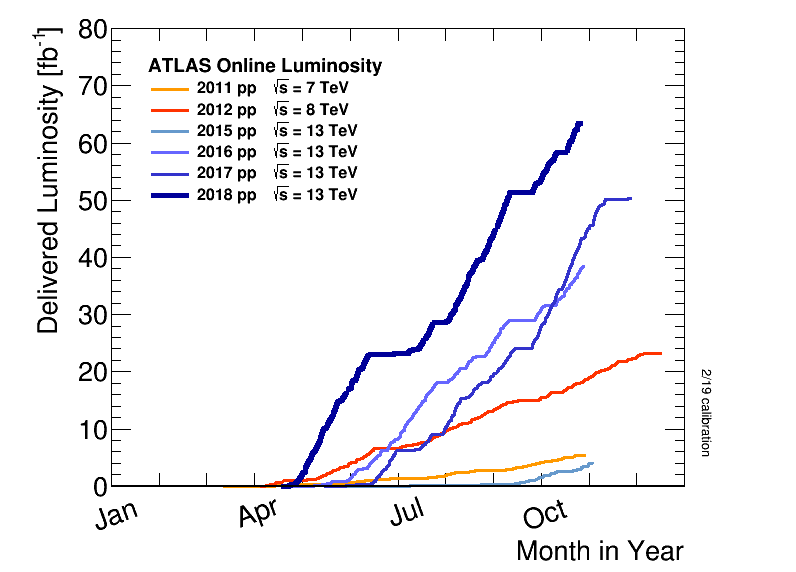
\includegraphics[scale=0.27]{ATLAS_Luminosity_Time.png}
				\caption{Delivered luminosity vs. time}
				\label{Fig:SFigATLASLuminosityTime}
			\end{subfigure}
			\begin{subfigure}{.49\textwidth}
				\centering
				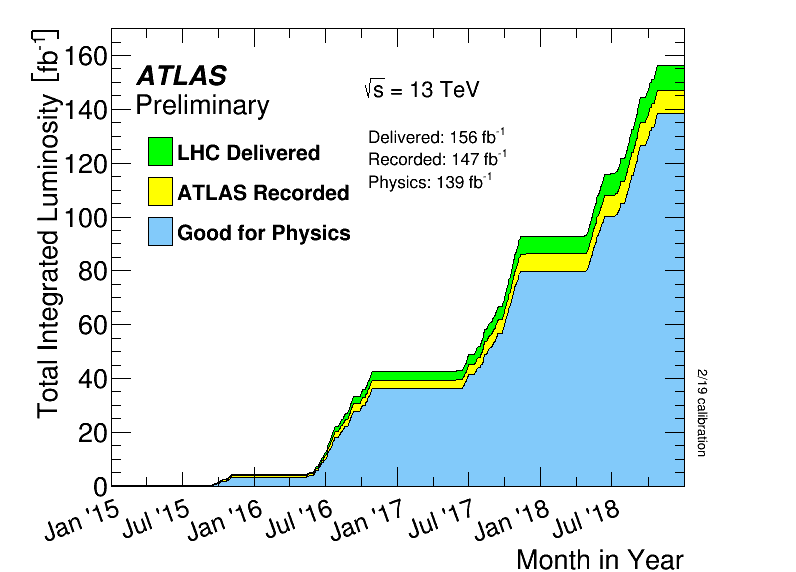
\includegraphics[scale=0.27]{ATLAS_Luminosity_Total.png}
				\caption{Total integrated luminosity vs. time}
				\label{Fig:SFigATLASLuminosityTotal}
			\end{subfigure}
			\caption{ (a) Cumulative luminosity versus month delivered to ATLAS during stable beams and for high energy \textit{pp} collisions. (b) Cumulative luminosity versus time delivered to ATLAS (green), recorded by ATLAS (yellow), and certified to be good quality data (blue) during stable beams for \textit{pp} collisions at 13 TeV centre-of-mass energy in 2015-2018 \cite{ATLASLumiPublic}.}
			\label{Fig:ATLASLuminosity}
		\end{figure}

		%01/02/21

		\subsection{Pileup}\label{Section:Pileup}

		In the collision of two nominally filled bunches there are a total of $2.3 \times 10^{11}$ protons available to collide, allowing a high number of hard $pp$ interactions. Ideally the experiments at CERN would only record these hard interactions however this is not always the case, as additional interactions between bunches can occur. These additional interactions are referred to as pileup and can cause a multitude of issues in the reconstruction of hard events such as track mis-reconstructions, degradation of object resolution, and ambiguity in primary vertex location. \par
		
		Pileup can be categorised into two types:

		\begin{itemize}
			\item \textbf{In-time} pileup refers to other interactions within \textit{the same} bunch as the hard interaction.
			\item \textbf{Out-of-time} pileup refers to interactions within \textit{other} bunches relative to the hard interaction.   
		\end{itemize}

		Pileup is quantified by use of $\left\langle \mu \right\rangle$, the average number of interactions per bunch crossing. This value is corresponds to the mean of the poisson distribution of the number of interactions per crossing calculated for each bunch, calculated from the instantaneous per bunch luminosity which is given by the equation:

		\begin{equation}
			\mu = \frac{\mathcal{L}_{bunch}\times\sigma_{inel}}{f}
		\end{equation}

		where $\mathcal{L}_{bunch}$ is the per bunch instantaneous luminosity, $\sigma_{inel}$ is the inelastic cross section (taken to be 80 mb for $\sqrt{s}=13 TeV$ collisions), and $f$ is the LHC revolution frequency of 11.245 kHz. The full pileup profile of Run 2
		can be seen in Figure \ref{Fig:ATLASPileup}. The pileup profile uses the full 146.9fb$^{-1}$ of online data recorded by ATLAS during Run 2 as opposed to the 139.9fb$^{-1}$ of physics data, which can be seen in Figure \ref{Fig:SFigATLASLuminosityTotal}. 

		\begin{figure}
			\centering
			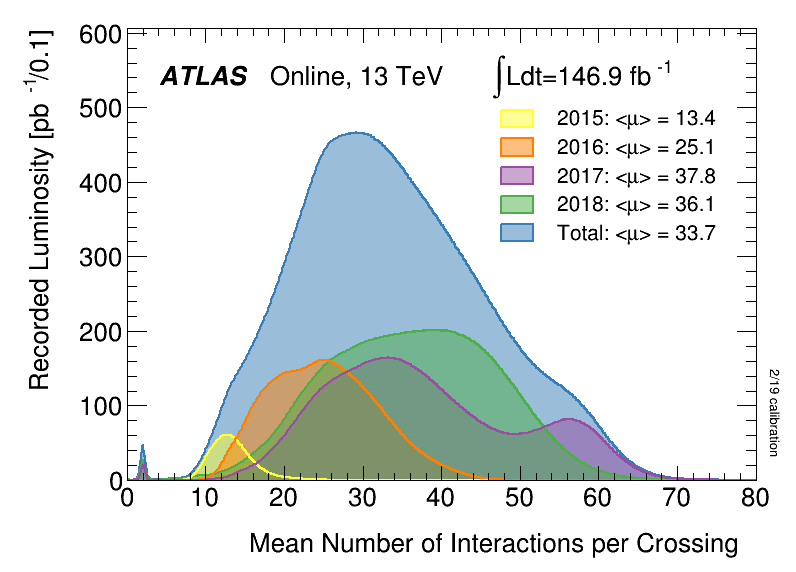
\includegraphics[scale=0.4]{ATLAS_Pileup_Run2.png}
			\caption{A figure showing the average interactions per bunch crossing for all ATLAS data recorded during Run 2 \cite{ATLASLumiPublic}.}
			\label{Fig:ATLASPileup}
		\end{figure}

		\section{ATLAS}

		The ATLAS (A Toroidal LHC ApparatuS) experiment \cite{ATLAS_Collab}, located at Point 1 of the LHC ring, is the largest general-purpose experiment at CERN. The design of ATLAS is carefully engineered in order to maximise its capabilities as a general-purpose particle detector \cite{ATLAS-TDR-01, ATLAS-TDR-02, Article:ATLASDesignPaper}. ATLAS is cylindrical in shape, with a length of 46 metres and a diameter of 25 metres. The immense scale of ATLAS can be difficult to picture without adequate reference: the diameter of ATLAS is 1 metre greater than the height of Buckingham palace, and its length is the same as the Statue of Liberty's height\footnote{The statue of liberty itself, excluding the 47 m pedestal that the statue stands upon.}. It would take a tower of 9 giraffes carefully lying head to hoof in the ATLAS cavern while wearing the appropriate personal protective equipment (PPE) to occupy the same length as the ATLAS detector\footnote{This would likely irritate the giraffes.}. 

		%02/02/21

		The ATLAS detector is constructed around the LHC beamline at Point 1 with its cylindrical geometry divided into two categories: the \textit{barrel} and the \textit{end-cap}, which can be visualised as the sides and top/bottom of a standard cylinder respectively. The cylindrical design of the ATLAS detector allows almost full coverage of 4$\pi$ and forward-backward symmetry across the IP, hence the IP is located at the perfect centre of the barrel region in the heart of the detector. Particles originating from collisions at the IP travel outward and through different sub-systems, each sensitive to particular properties of various particles, in order to identify and reconstruct physics objects in each event. \par 

		%03/02/21

		The \hyperref[Section:InnerDetector]{Inner Detector (ID)}, the sub-system closest to the IP, tracks the path of all charged particles that pass through it. For particles travelling outward from the IP the next sub-system encountered are the \hyperref[Section:Calorimeters]{ATLAS Calorimeters} which aim to stop both hadronic and electromagnetic particles in order to measure their energy. Finally, the remaining particles from events at the IP pass through the outermost sub-system: the Muon Spectrometer (MS), which aims to identify and track the path of muons. All of these systems are subjected to a magnetic field generated by the ATLAS magnet systems: a solenoid magnet creates the field beyond the ID, and the eponymous toroidal magnet creates the magnetic field beyond the calorimeters. A cross section of ATLAS and these detector sub-systems can be seen in Figure \ref{Fig:ATLASDetector}.

		\begin{figure}
			\centering
			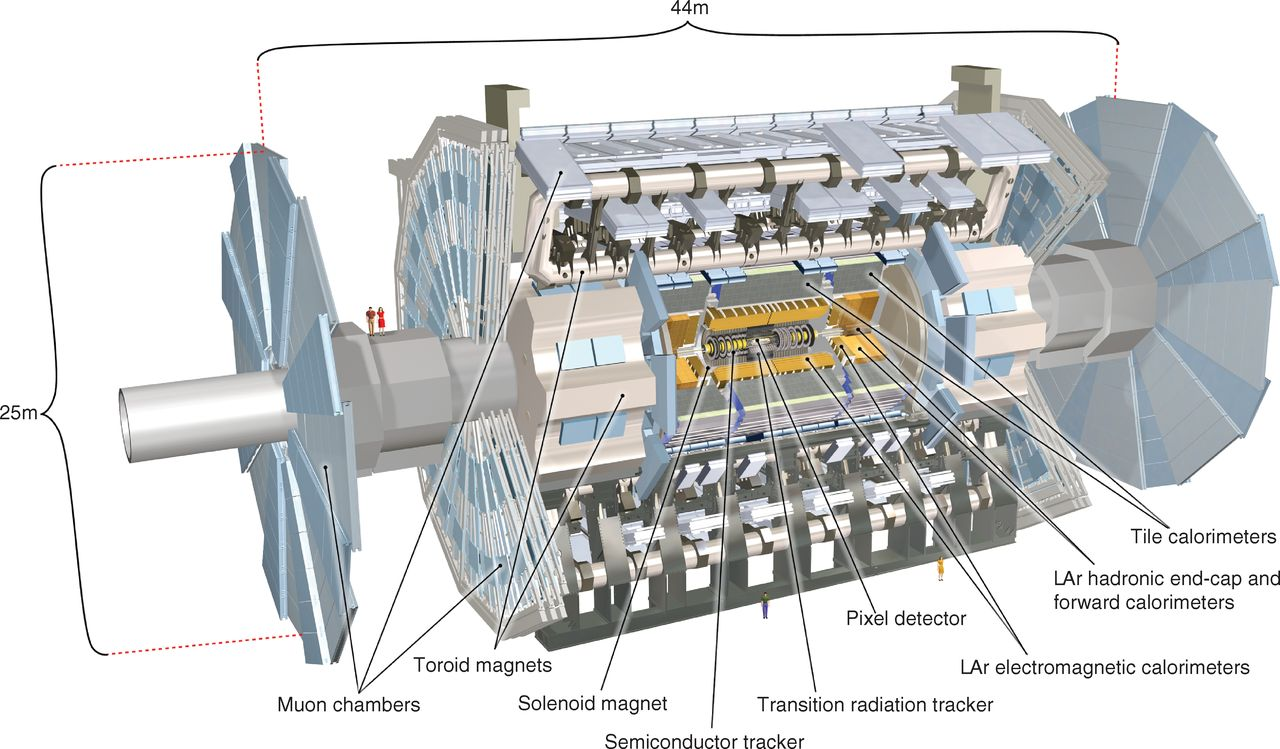
\includegraphics{ATLAS}
			\caption{A figure showing the subsystems of the ATLAS detector \cite{Article:ATLASDesignPaper}.}
			\label{Fig:ATLASDetector}
		\end{figure}

		\subsection{The ATLAS Coordinate System}

		In order to be able to accurately describe events relative to the detector and interaction point, ATLAS uses a well defined right-handed coordinate system. Taking the nominal IP as the origin, the $x$-axis points towards the centre of the LHC ring, the $y$-axis points vertically upwards, and the $z$-axis points along the direction of the beam pipe. A subtle yet crucial result of this coordinate system is the definition of the $x$-$y$ plane, which is tangential to the beam pipe (referred to as the \textit{transverse} plan). The nature of the fundamental colliding partons prevent the initial momentum in the $z$ direction from being known, however it is known that the partons have zero initial momentum in the transverse plane and therefore directional vector quantities such as momenta can be projected into the transverse plane. \par

		In addition, cylindrical coordinates are used to describe the geometry of the detector. The azimuthal angle, $\phi$, describes the angle around the beam direction in the transverse plane where $\phi = 0$ points in the same direction as the $x$-axis (i.e. towards the centre of the LHC ring). The polar angle, $\theta$, describes the angle from the beam direction in the $y$-$z$ plane where $\theta = 0$ points in the same direction as the $y$ axis (i.e. along the beam pipe). The final coordinate of the ATLAS coordinate system is the rapidity ($y$) or pseudorapidity ($\eta$). The rapidity of a particle is defined as: 

		\begin{equation}
			y = \frac{1}{2}\ln\left(\frac{E+p_{z}}{E-p_{z}}\right)
		\end{equation}

		where E is the particle's energy and $p_{Z}$ is the momentum of the particle in the $z$ axis. The pseudorapidity of a particle is defined in terms of the polar angle, $\theta$, as:

		\begin{equation}
			\eta = -\ln\tan\left(\frac{\theta}{2}\right)
		\end{equation}

		Pseudorapidity is typically used in place of $\theta$ as it is Lorentz invariant under a boost in the $z$-axis whereas $\theta$ is not. The rapidity and pseudorapidity are equivalent for massless particles and this holds true for particles with extremely small mass (several orders of magnitude lower than their average energy) such as electrons. The angular distance between two objects is described using the variable $\Delta R$, which is also Lorentz invariant under a boost in the $z$-axis. $\Delta R$ is defined by the relation:

		\begin{equation}
			\Delta R = \sqrt{ (\Delta\eta)^{2} + (\Delta\phi)^{2} }
		\end{equation}

		%04/02/21

		\subsection{The Magnet System}\label{Section:Magnets}

		The ATLAS magnet system consists of four magnets: a single solenoid magnet \cite{ATLASSolenoidMagnet}, and three toroidal magnets \cite{ATLASBarrelToroid, ATLASEndcapToroid} (which contribute an important part of the ATLAS name). The central solenoid provides the magnetic field for the inner detector, and the toroidal magnets provide the magnetic field	for the muon system. The arrangement of the magnet systems within ATLAS can be seen in Figure . \par

		\begin{figure}
			\centering
			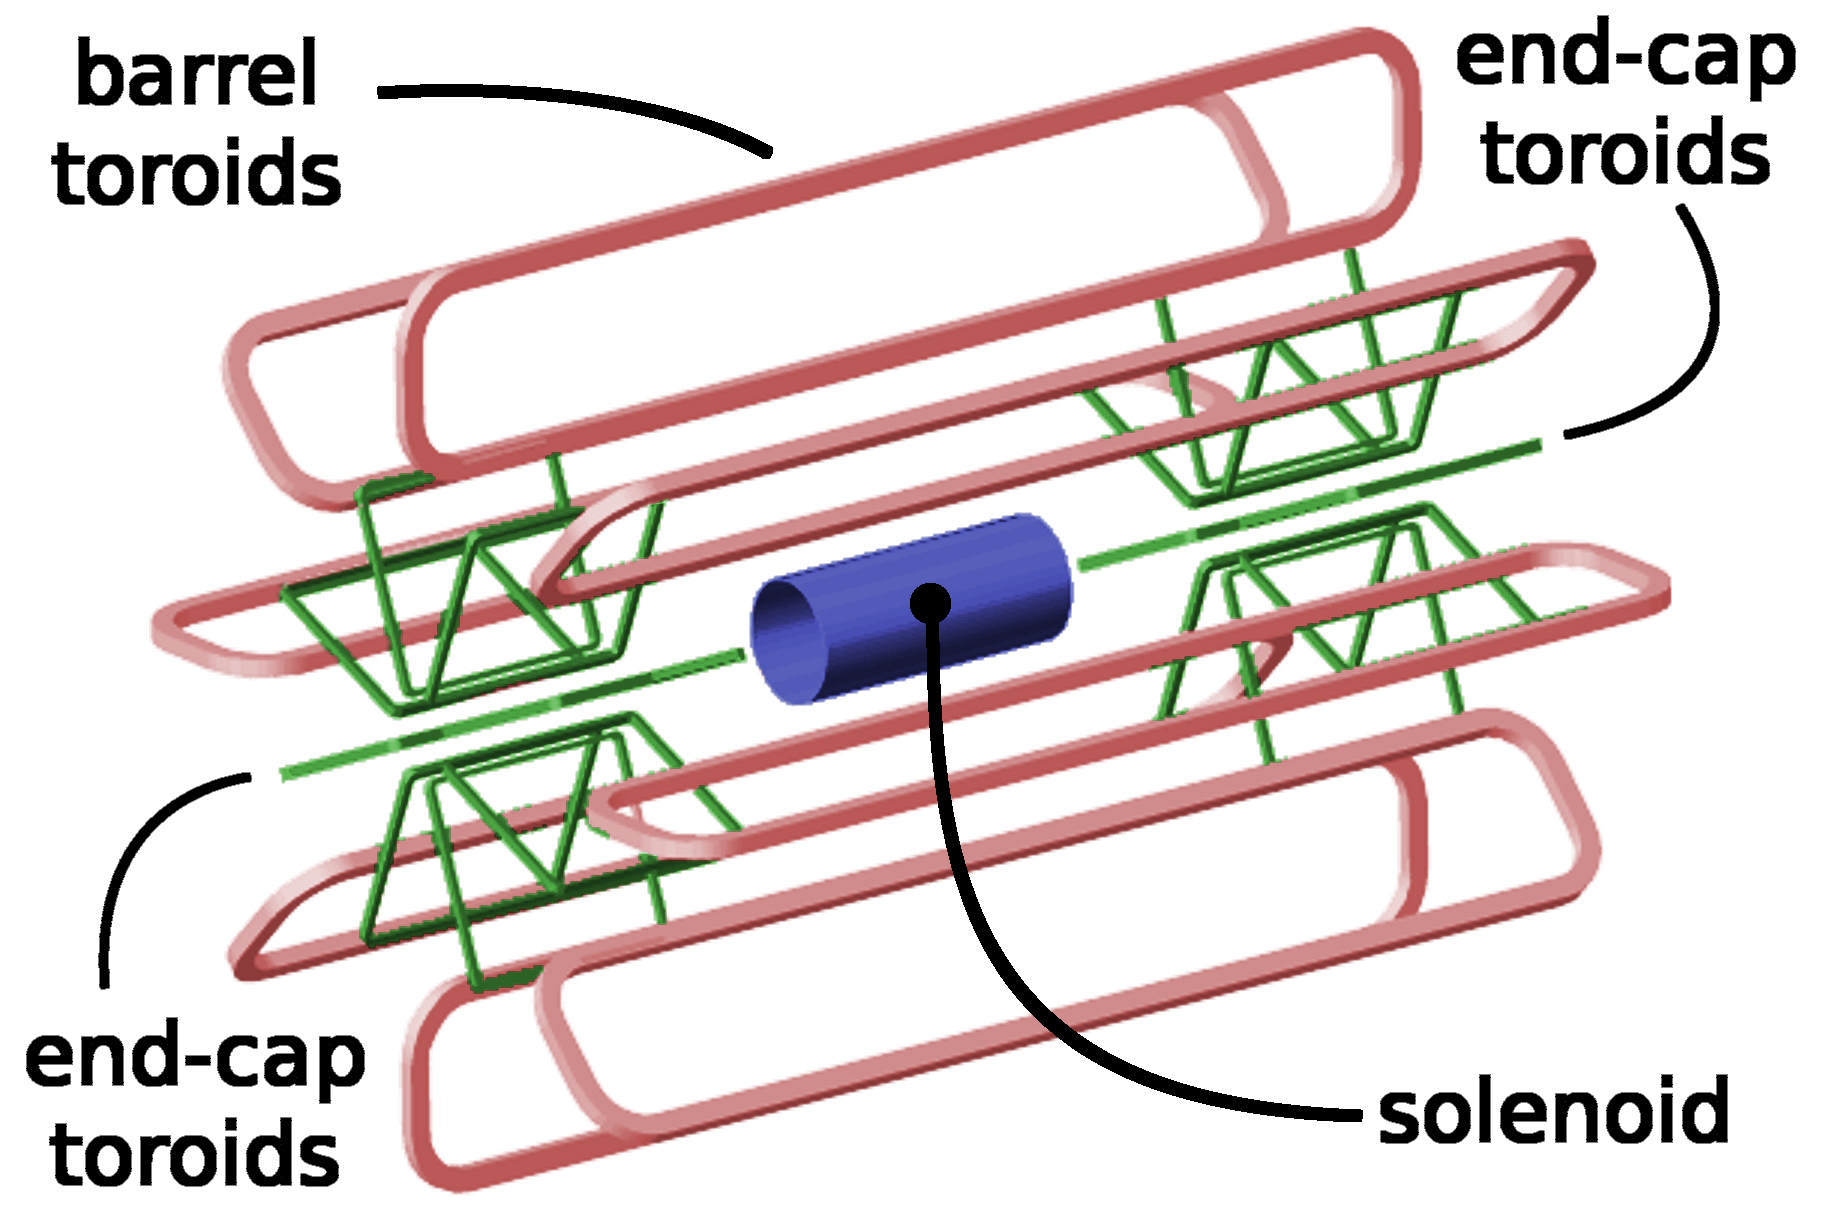
\includegraphics[scale=0.15]{Magnet_Layout.png}
			\caption{The relative location of the solenoid, barrel toroids, and end-cap toroids \cite{ATLASToroids}. }
			\label{Fig:CernMagneticLayout}
		\end{figure}

		The solenoid magnet is named the Central Solenoid Magnet. It is aligned with the $z$-axis (i.e. the beam pipe) and exerts a 2T axial magnetic field which bends the path of charged particles within the inner detector. The magnet weighs 5 tonnes but is only 5 cm thick (which corresponds to 0.66 radiation lengths) in order to minimize the probability of particle interactions with the magnet itself. The solenoid is cooled to a temperature of 4.5 K in order to maintain its superconducting state, and is capable of storing a total of 38 MJ of energy. \par
		
		In the case of the toroidal magnets, there is one toroidal magnet located in the barrel region and one toroidal magnet in each end-cap region. The magnetic fields produced by the toroids are orthogonal to each other, creating an overall magnetic field of 0.5 T in the barrel region and 1 T in each end-cap. Together, these magnetic fields bend the path of muons in the outermost region of the detector. The position of each toroid's coils can be seen in Figure \ref{Fig:CernMagneticLayout}. Each magnet contains eight coils, however the coils for the barrel region are by far the largest with a length of 25.3 metres each whereas the length of the end-cap coils are only 5 metres. Each end-cap toroid weighs 240 tonnes and stores 0.25 GJ of energy, while the much larger barrel toroid weights a total of 830 tonnes and stores a total of 1.08 GJ of energy. 
		
		The shape of the magnetic field created within ATLAS by both the solenoid and toroidal magnet can be seen in Figure \ref{Fig:CernMagneticField}. 
		
		\begin{figure}
			\centering
			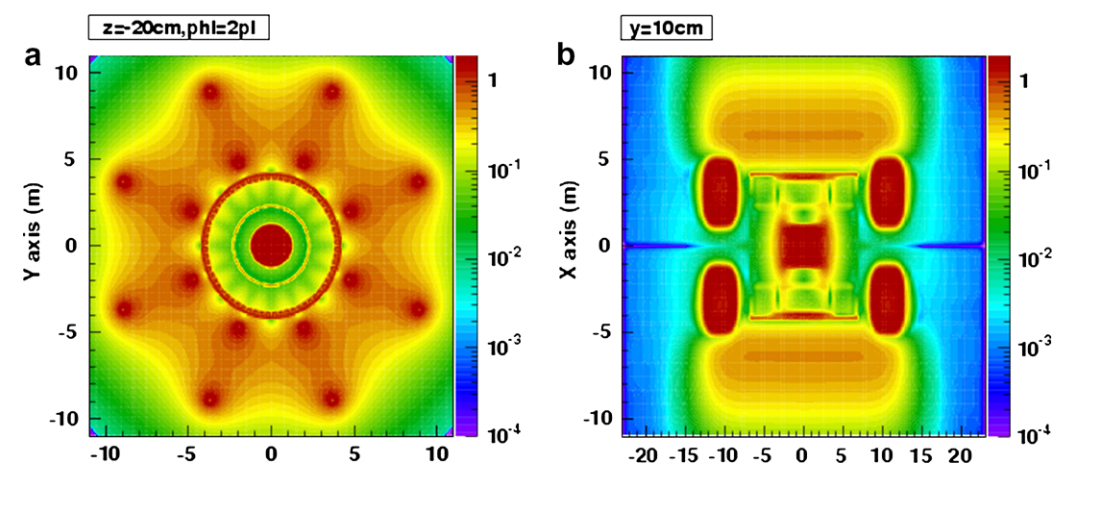
\includegraphics[scale=0.4]{Magnetic_Field}
			\caption{The shape of the magnetic field within the ATLAS detector. The left plot shows the magnetic field as if looking down the beamline. The right plot shows the magnetic field when viewed from above \cite{Article:CernMagnets}. }
			\label{Fig:CernMagneticField}
		\end{figure}

		% 05/02/21

		\subsection{The Inner Detector}\label{Section:InnerDetector}

		The Inner Detector \cite{ATLASID1, ATLASID2} is the most central component of ATLAS providing precise measurements of both particle charge and momentum, in addition to tracking charged particles to a pseudorapidity range of $|\eta| < 2.5$. Using both an impact parameter, $d_{0}$, and a longitudinal impact parameter, $z_{0}$, the ID is able to characterise the primary vertex of each interaction. The parameter $d_{0}$ is defined as the distance between the vertex's point of closest approach and the $z$-axis, and the parameter $z_{0}$ is defined as the $z$-coordinate of the primary vertex's point of closest approach. A high precision measurement of the primary vertex is crucial to this analysis as the delayed secondary vertex of b-tagged events is an extremely important in their identification, and an excellent resolution for $d_{0}$ and $z_{0}$ allows for easier identification of b-hadrons and other particles with longer lifetime. The layout of these components within the ID barrel region can be seen in Figure \ref{Fig:InnerDetector}.  

		The ID consists of four subsystems which work in conjunction to track charged particles and perform high resolution measurements of their charge and momentum. These subsystems are the \hyperref[Section:IBL]{Insertable B-Layer (IBL)}, the \hyperref[Section:PixelDetector]{Pixel Detector}, the \hyperref[Section:SCT]{Semiconductor Tracker (SCT)}, and the \hyperref[Section:TRT]{Transition Radiation Tracker (TRT)}. A cross section of these systems within the ID can be seen in Figure \ref{Fig:InnerDetectorXsec}.

		\begin{figure}
			\centering
			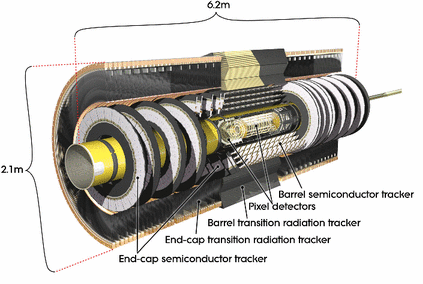
\includegraphics[scale=0.7]{Inner_Detector}
			\caption{A figure showing a cut-away view of the ATLAS inner detector and its components \cite{ATLASIDImage}. }
			\label{Fig:InnerDetector}
		\end{figure}

		\begin{figure}
			\centering
			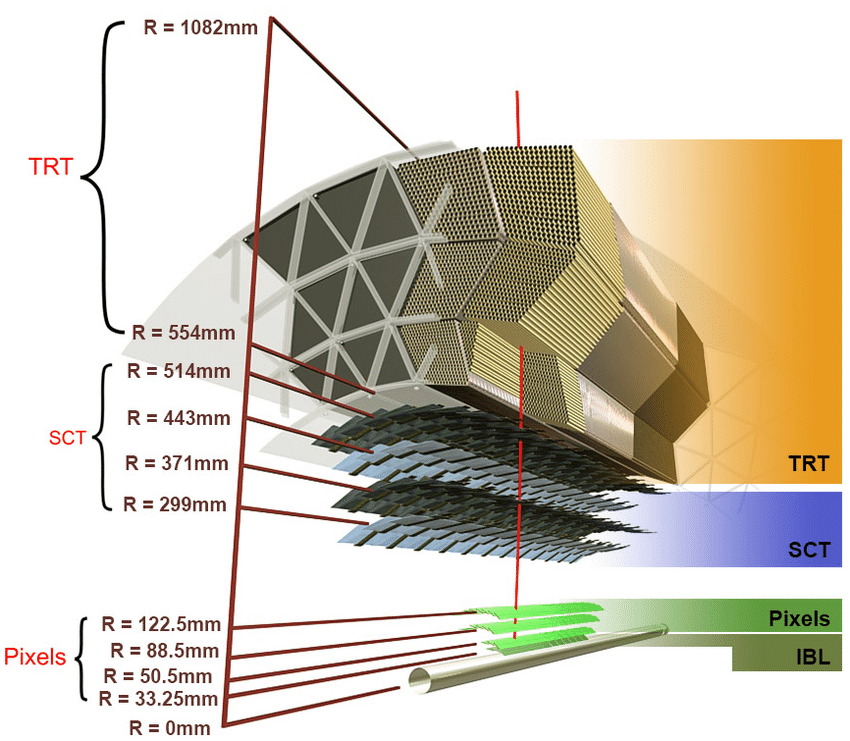
\includegraphics[scale=0.4]{ATLAS_ID_Layers}
			\caption{A figure showing a cross section of the ATLAS inner detector barrel region and its components \cite{ATLASIDImage}.}
			\label{Fig:InnerDetectorXsec}
		\end{figure}

		The IBL, pixel detector, and SCT all operate through the use of pixel modules containing tens of thousands of silicon pixel sensors. As charged particles pass through the pixel sensors, they ionise with the silicon semiconductors, freeing electrons from atoms within the silicon and creating ion-electron pairs. By interpreting the resultant signal created at the points within these pixel modules that these ion-electron pairs are created, the path of the charged particles that pass through the ID can be measured. 

		\subsubsection{The Insertable B-Layer (IBL)}\label{Section:IBL}

		The most central component of the ID is the IBL \cite{IBL-TDR} (positioned a mere R = 33.25 mm away from the beam pipe), which was added to ATLAS during the shutdown between Run 1 and Run 2. The IBL increases the resolution of $d_{0}$ and vertex measurements when compared with the pixel detector alone, which is an important addition due to the high pileup of Run 2 (which can easily obfuscate the primary vertex as discussed in Section \ref{Section:Pileup}). Each individual pixel is extremely small and has dimensions of $50 \mu m \times 250 \mu m$, which allows for a tracking resolution of 8 $\mu$m and 40 $\mu$m in the $x$-$y$ plane and $z$ direction respectively.  

		\subsubsection{The Pixel Detector}\label{Section:PixelDetector}

		The pixel detector consists of three layers of concentric cylinders coaxial to the beam pipe, and three layers of end-cap disks perpendicular to the beam pipe. The barrel layers are positioned at R = 50.5, 88.5, and 122.5 mm, with the end-cap disks positioned at $z$ = 495, 580, and 650 mm. These components consist of a total of 1744 pixel modules \cite{ATLASPixel} with a thickness of 250 $\mu$m, each containing 47,232 pixels with dimensions of 50 $\mu$m $\times$ 400 $\mu$m. Each pixel module contains 16 front-end chips with 2880 readout channels equating to a total of 46,080 readout channels per module, however all 47,232 pixels are readout of each module (pixels in the inter-chip regions are ganged together to be readout). Overall, the pixel detector has over 80 million readout channels and provides a spatial resolution of 10 $\mu$m in the $x$-$y$ plane and a spatial resolution of 115 $\mu$m in the $z$-axis. 

		% 08/02/21

		\subsubsection{The Semiconductor Tracker (SCT)}\label{Section:SCT}

		The Semiconductor Tracker (SCT) \cite{ATLASSCT} sits outside the pixel detector and is similar in operation, consisting of 4 barrel layers and 9 end-cap disks. The barrel layers are positioned at R = 299, 371, 443, and 514 mm, and the end-cap disks range from $z$ = 854 - 2720 mm. The 15,912 strip modules have a thickness of 285 $\mu$m and consist not of pixels as per the pixel detector but 768 silicon strips each 12 cm long, necessitating over 6.4 million readout channels. In total the SCT contains 61 m$^{2}$ of silicon strip sensors, and provides a hit resolution of 17 $\mu$m in the $x$-$y$ plane and a hit resolution of 580 $\mu$m in the $z$-axis. 

		\subsubsection{The Transition Radiation Tracker (TRT)}\label{Section:TRT} 

		The Transition Radiation Tracker (TRT) \cite{ATLASTRT} is the furthest component of the ID from the beam pipe, with a barrel region positioned at 563 $<$ R $<$ 1066 mm and $|z| <$ 712 mm and two end-caps at 644 $<$ R $<$ 1004 mm and 848 $< |z| <$ 2710 mm. The method of detection used by the TRT differs from the previous ID modules: instead of using silicon semiconductors, the TRT consists of thin-walled proportional drift tubes called "straws" containing a nominal mixture of 70\%/27\%/3\% xenon/carbon dioxide/oxygen gas. \par 

		In addition to being filled with this gas mixture, each straw contains a central gold-plater tungsten wire of diameter 32 $\mu$m and has a potential applied between the central wire and outer wall of the drift tubes. When charged particles pass through the straws, atoms within the gas are ionized and drift towards the walls of the straws while electrons drift towards the wire. The wire amplifies the signal of these electrons by a factor of approximately 20,000 by releasing an avalanche of electrons which creates an interpretable signal and allows the extraction of timing information. \par

		Additional ionization can occur from transition radiation photons which originate from the thin material between straws made of polypropylene and polyethylene fibres. Incoming charged particles moving between media with differing refraction indexes have a probability of emitting these transition radiation photons with energies proportional to their Lorentz factor. This interaction is exploited during electron identification as electrons will have higher Lorentz factors (and therefore create a larger pulse within the wire) than many other charged particles such as muons and pions. \par

		The TRT consists of 52,544 coaxial straws of length 144 cm ie barrel region and 122,880 radial straws of length 37 cm in each end-cap, totalling almost 300,000 straws across the entire TRT. Due to these numbers and the geometry of ATLAS, charged particles are guaranteed to cross 35-40 straws in a pseudorapidity interval of $|\eta| < 2$. Overall, the TRT provides a hit resolution of 130 $\mu$m per straw \cite{ATLASTRTRes}. 

		\subsection{The Calorimeters}\label{Section:Calorimeters}

		Calorimeters are instruments that measure the energy of particles: incoming particles are absorbed by the calorimeter and deposit their full energy which is converted into a measurable signal. The calorimeter system within ATLAS uses two main types of calorimeters: electromagnetic calorimeters for energy measurements of electromagnetic particles, and hadronic calorimeters for energy measurements of hadronic particles. These calorimeters measure all SM particles excluding muons and neutrinos, with a coverage up to $|\eta| < 4.9$. The layout of these calorimeters within ATLAS can be seen in Figure \ref{Fig:ATLASCalorimeters}. \par

		The ATLAS calorimeters are \textit{sampling} calorimeters which operate using an alternating pattern of layers of an absorber medium and an active medium. Incoming particles interact within the absorber medium which decreases their energy and creates a shower of secondary particles that subsequently interacts within the active medium to produce a detectable signal.  

		\begin{figure}
			\centering
			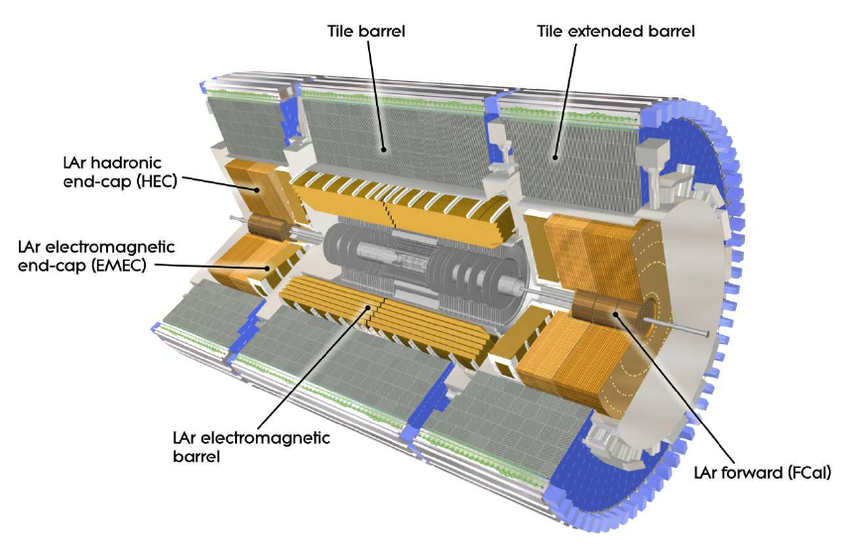
\includegraphics[scale=0.4]{ATLAS_Calorimeters}
			\caption{A figure displaying the arrangement of the electromagnetic and hadronic calorimeters within the ATLAS detector \cite{AtlasCalImage}.}
			\label{Fig:ATLASCalorimeters} 
		\end{figure} 

		\subsubsection{The Electromagnetic Calorimeter}\label{Section:ECal}

		The electromagnetic calorimeter or LAr calorimeter \cite{ATLASECalTDR} has the primary function of measuring the energy of electrons and photons in the pseudorapidity region $|\eta| < 3.2$. Lead is chosen as the absorber material, with liquid argon (LAr) as the active material. Two main processes occur within the lead absorber material that lead to showering and a measurement of incoming particle energy:
		
		\begin{itemize}
			\item \textit{Bremsstrahlung}, where incoming electrons interact with the lead atoms' dense nucleus to lose kinetic energy which is emitted as bremsstrahlung photons.
			\item \textit{Pair production}, where a photon is converted to an electron-positron pair.
		\end{itemize}

		Incoming particles will rapidly alternate between bremsstrahlung and pair production, depositing energy within the LAr active material each time. This process is called \textit{showering}, and continues until the shower no longer has enough energy to produce further particles (i.e. the electron does not have enough kinetic energy to radiate as a photon or the photon no longer passes the energy threshold for electron-positron pair production). At this point, the particles continue losing their energy through more simple mechanisms until they come to a complete loss (via physical collisions with atoms for electrons and compton scattering/the photoelectric effect for photons). \par

		These are not the only mechanisms through which EM particles can deposit energy within the EM calorimeter (for example pions are capable of producing a photon pair), however they are among the most common. It is important to note that muons also produce small energy deposits in the EM calorimeter, however due to the nature of muons as minimally ionising particles this is often simply the radiation of a low energy photon. These low energy photons may shower and produce low energy showers, however these are often easily distinguishable from the higher energy showers of electrons and photons. Following the shower produced by an incoming particle, ionisation electrons within the LAr active material will drift towards a copper electrode (similarly to the system explained in \ref{Section:TRT}) in order to produce a measurable signal. \par
		
		The EM calorimeter consists of a barrel calorimeter providing coverage in the pseudorapidity range $0 < |\eta| < 1.475$ and two end-cap calorimeters providing coverage in the pseudorapidity range $1.375 < |\eta| < 3.2$. The geometry of the EM calorimeter uses a unique accordion-shaped geometry which allows for a completely hermetic design (i.e. no gaps of any kind are required between the absorber and active materials for devices such as readout systems). The readout of the EM calorimeter can occur from either the front or back, which allows for full coverage in $\phi$. The accordion geometry of the EM calorimeter can be seen in Figure \ref{Fig:ATLASECalAccordion}. 

		\begin{figure}
			\centering
			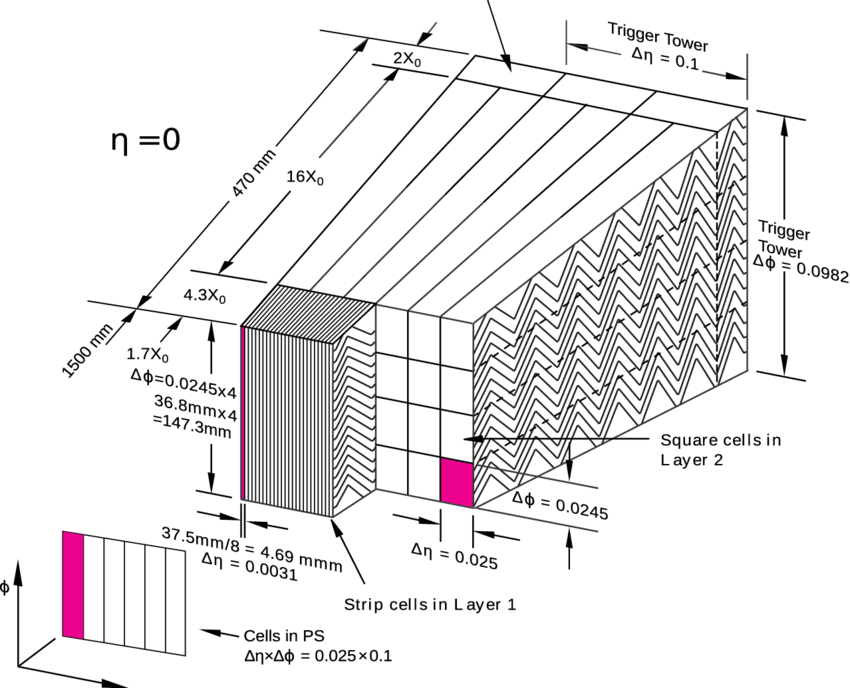
\includegraphics[scale=0.4]{ATLAS_EMCal_Accordion}
			\caption{A figure showing the unique accordion shape of the ATLAS EM calorimeter \cite{ATLASECalAccordionImage}.}
			\label{Fig:ATLASECalAccordion}
		\end{figure}

		To perform the best possible energy measurement of an incoming particle, the particle must be completely stopped within the medium of the calorimeter. A greater calorimeter length increases the probability of completely stopping an incident particle, however additional length beyond what is required to stop the incident particle is inefficient in terms of maintenance, power, and cost. In order to find this ideal balance of calorimeter length the radiation length, $X_{0}$, is used to characterise the behaviour of the incident EM showers. $X_{0}$ is defined as the distance within a given material that an incident photon or electron must travel in order to lose $1/e$ of its energy.  In total the EM calorimeter has a depth of over 22 $X_{0}$ composed of three layers of varying depth, $X_{0}$, and $\eta$/$\phi$ granularity plus an additional zeroth layer called the presampler \cite{ATLASECalAccordionImage}. \par

		% 09/02/21		

		These layers are:

		\subparagraph{The presampler (PS) layer,} a relatively thin cluster of LAr layers only (i.e. no absorber material) separate from the calorimeter and positioned before some infrastructure components. The aim of the PS layer is to estimate the total loss of energy upstream of the calorimeter due to material interactions (within the inner detector, cryostat, and solenoid coil up to $|\eta| < 1.5$). The PS layer is only 11 mm thick in the barrel region and only 5 mm thick in the end-caps, covering a pseudorapidity range of $|\eta| < 1.8$.
		
		\subparagraph{Layer 1,} which has a thickness of 4.4 $X_{0}$ at $\eta = 0$ and is segmented into strips with varying granularity across $\eta$. For $|\eta| < 1.4$ and $1.5 < |\eta| < 2.4$ these are high granularity segmentation, whereas for the range of $1.4 < |\eta| < 1.5$ and $2.4 < |\eta| < 2.5$ the segmentation is coarser. The purpose of this differing granularity is to allow for discriminating power between photon showers caused by single photons, and showers from two collimated photons decaying from neutral hadrons (such as in the case of a neutral pion producing two photons). The cells in the finer granularity $\eta$ region have the size of $0.003 \times 0.0982$ in $\Delta\eta \times \Delta\phi$, and the cells in the coarser $\eta$ region have a size of $0.025 \times 0.0982$ in $\Delta\eta \times \Delta\phi$. 
		
		\subparagraph{Layer 2,} which has a thickness of 16 $X_{0}$ where the bulk of energy depositing occurs. The cells in this layer have a size of $0.025 \times 0.0245$ in $\Delta\eta \times \Delta\phi$. 
		
		\subparagraph{Layer 3,} which has a thickness of 2 $X_{0}$ designed to measure and correct for the leakage of higher energy calorimeter showers beyond the EM cal and potentially into the hadronic calorimeter. The cells in this layer have a size of $0.05 \times 0.0245$ in $\Delta\eta \times \Delta\phi$. 
		
		\subsubsection{The Hadronic Calorimeter}\label{Section:HCal}

		Just as the EM calorimeter performs energy measurements of incoming EM particles, the hadronic calorimeter or Tile calorimeter \cite{ATLASTileTDR} measures energies of incoming hadronic particles in the region of $|\eta| < 4.9$. The Tile calorimeter consists of three barrel layers and two wheels per end-cap, each using differing absorber and active materials:
		
		\begin{itemize}
			\item The barrel region uses plates of steel as its absorber material and plastic scintillator tiles as its active material.
			\item The hadronic end-cap (HEC) in the end-cap region $1.5 < |\eta| < 3.2$ uses copper as its absorber material and LAr as its active material. 
		\end{itemize}

		Interactions with the steel nuclei in the barrel region cause particle showers containing charged particles that interact with the scintillating active material in order to produce ultraviolet scintillation photons. These photons are carried to photomultiplier tubes (PMTs) via wavelength shifting fibres which convert the photons into a measurable electronic signal. A larger interaction within the scintillation tiles produces a stronger signal, and so measuring the intensity of the signal allows for a measurement of energy deposited by the incident hadronic particle. \par

		Hadronic showers are characterised by the \textit{interaction length} which defined as the distance between interactions within a given material to reduce the number of relativistic charged particle by a factor of $1/e$. Hadronic showers occur via the strong interaction typically producing wider showers mainly consisting, allowing for coarser granularity than in the EM calorimeter. \par

		The barrel region of the hadronic calorimeter has a depth of 9.7 $\lambda$ and cell sizes of $0.1 \times 0.1$ in $\Delta\eta \times \Delta\phi$ for the first two layers, and $0.2 \times 0.1$ in $\Delta\eta \times \Delta\phi$ in the last layer. The end-cap wheels have a depth of 10 $\lambda$ and similar granularity to the barrel region of  $0.1 \times 0.1$ in $\Delta\eta \times \Delta\phi$ in the first wheel, and $0.2 \times 0.1$ in $\Delta\eta \times \Delta\phi$ for the second. 

		\subsubsection{The Forward Calorimeter}\label{Section:FCal}

		ATLAS uses an additional calorimeter in the forward region of $3.2 < |\eta| < 4.9$ in order to increase the calorimeter coverage within ATLAS up to the pseudorapidity range of $|\eta| < 4.9$. The forward calorimeter (FCal) is a sampling calorimeter capable of performing energy measurements of both EM and hadronic particles via its use of a combination of multiple absorber materials. \par
		
		The FCal has a depth of 10 $\lambda$ and is segmented into three layers: while the FCal consistently uses LAr as its active material, the first layer uses copper layers as its absorber material in order to perform measurements of EM particles before switching to a tungsten absorber material in the second and third layers for hadronic energy measurements.  

		\subsection{The Muon Spectrometer}\label{Section:MuonSystem}

		The final and outermost subsystem of the ATLAS detector is the Muon Spectrometer (MS) \cite{ATLASMuonTDR}. Interspersed between the toroidal magnet, the muon system is composed of two systems made up of pairs of triggering and tracking systems with the aim to track and measure muons in the pseudorapidity range of $|\eta| < 2.7$. Muons that pass through the system are subjected to ATLAS' magnetic field (discussed in Section \ref{Section:Magnets}), bending the muon tracks and allowing for muon momentum measurements. \par

		The MS can be divided into a barrel region in the pseudorapidity range of $|\eta| < 1.05$ and an end-cap region from $1.05 < |\eta| < 2.7$. Four main components in various configurations are used to provide the full functionality of the MS: \hyperref[Section:MDTs]{Monitored Drift Tubes (MDTs)} \cite{ATLASMDT}, \hyperref[Section:RPCs]{Resistive Plate Chambers (RPCs)} \cite{ATLASRPC}, \hyperref[Section:CSCs]{Cathode Strip Chambers (CSCs)} \cite{ATLASCSC}, and \hyperref[Section:TGCs]{Thin Gap Chambers (TGCs)} \cite{ATLASTGC}. The positioning of each of these components can be seen in Figure \ref{Fig:MuonSystem}. 

		\begin{figure}
			\centering
			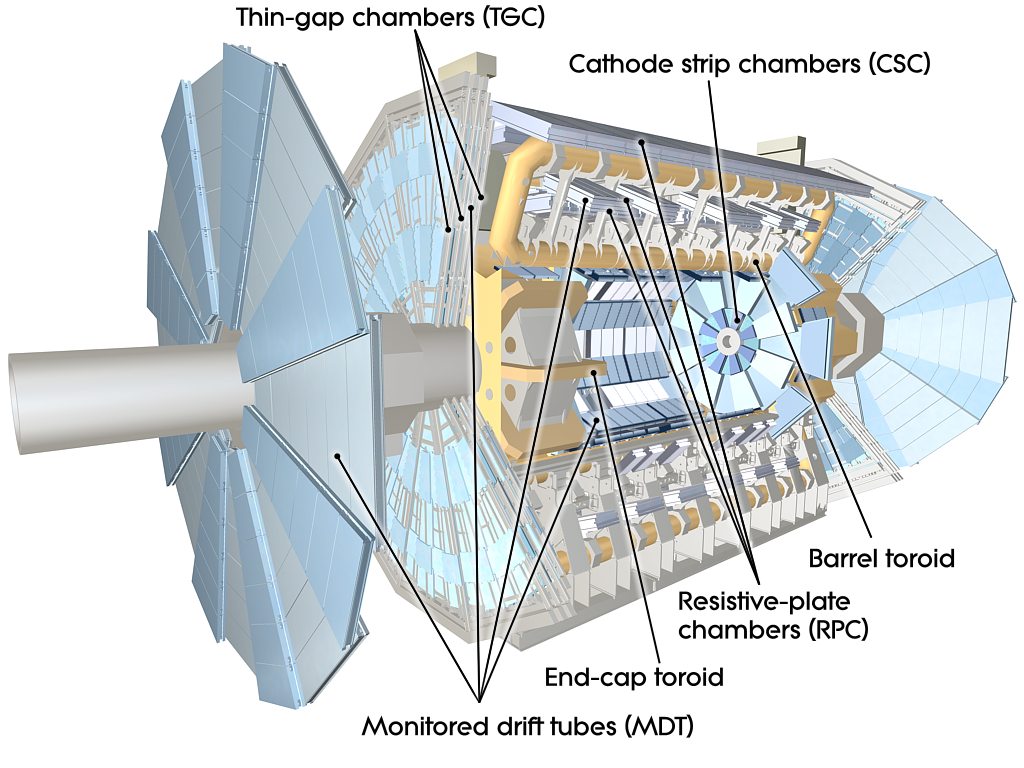
\includegraphics[scale=0.3]{Muon_System}
			\caption{A figure showing the position of the individual muon systems within ATLAS \cite{Article:ATLASDesignPaper}.}
			\label{Fig:MuonSystem}
		\end{figure}

		\subparagraph{Monitored Drift Tubes (MDTs)}\label{Section:MDTs}\mbox{}\\
		MDTs can essentially be thought of as larger versions of the TRT straws discussed in Section \ref{Section:TRT}. They are drift tubes with a diameter of 3 cm containing a central wire made of tungsten and filled with argon gas, subjected to a potential between the tube wall and the wire. Muons ionise the argon gas within the MDTs, and the electrons drift towards the tungsten wire to produce a detectable signal. The drift time of the charge within the MDTs allows for attainment of a spatial precision of 80 $\mu$m.

		\subparagraph{Resistive Plate Chambers (RPCs)}\label{Section:RPCs}\mbox{}\\
		A single RPC unit contains two gas volumes bounded by two bakelite capacitor plates and separated by a grid of 2 mm spacers. The gas volume is filled with C$_{2}$H$_{2}$F$_{4}$ gas and subjected to a potential. Muons passed through the gas volume ionise the gas, and ionised electrons from these interactions are read out from the RPC unit allowing for a trigger timing resolution of 2 nanoseconds. 
		
		\subparagraph{Cathode Strip Chambers (CSCs)}\label{Section:CSCs}\mbox{}\\
		CSCs are multi-wire proportional chambers, which typically consist of equally spaced parallel wires sandwiched between cathode planes \cite{MultiwirePropChamber}. The remaining unit volume is filled with gas, which is ionised by incident charged particles. The CSCs uses alternating planes of tungsten wires and two segmented cathodes in a 80\%/20\% argon/carbon dioxide gas volume, with one set of cathode strips running perpendicular to the wires and the other set of strips running parallel to the wires. This configuration of the CSCs provides a resolution of 60 $\mu$m per layer. 

		\subparagraph{Thin Gap Chambers (TGCs)}\label{Section:TGCs}\mbox{}\\
		Much like the CSCs, the TGCs are also multi-wire proportional chambers. The key difference between the two is their slightly differing design: the TGCs use  50 $\mu$m gold plated tungsten wires and a 45\%/55\% n-pentane/carbon dioxide gas volume \cite{ATLASTGCCertification}. The TGCs allow for a faster timing resolution than the CSCs alone (approximately 4 ns compared with 7 ns). 

		The MS barrel uses a combination of MDTs and RPCs for tracking and triggering respectively. The barrel component of the MS consists of three cylindrical layers of MDTs, with RPCs surrounding the last two MDT layers. The end-cap region of the MS consists of four wheels containing MDTs and CSCs for tracking, and TGCs for triggering: the first wheel at higher pseudorapidity of $2.5 < |\eta| < 2.7$ uses CSCs in place of MDTs, as the occupancy of the MDTs is too high in this region. The remaining three wheels use MDTs, with three layers of TGCs surrounding the third wheel. The arrangement of the muon system can be seen in Figure \ref{Fig:MuonSystemLayout}. 

		\begin{figure}
			\centering
			\includegraphics[scale=1.5]{Muon_schematic_transp}
			\caption{A figure showing the arrangement of muon system components within the ATLAS detector \cite{ATLASTriggerImage}.}
			\label{Fig:MuonSystemLayout}
		\end{figure}

		%10/02/21

		\subsection{The ATLAS Trigger System}

		Attempting to record every interaction that occurs within the ATLAS detector is a herculean task. Bunches accelerated by the LHC cross every 25 ns, giving a frequency of 40 MHz. If each event has a raw size of 1.5 MB, ATLAS must record and store to disk 60 TB per second. The current record for highest data throughput attained experimentally is only 178.08 Tb or 22.25 TB per second \cite{UCLThroughput}, and was only achieved in July 2020 (over a year after the beginning of Long Shutdown 2). \par

		Fortunately, recording every single ATLAS interaction is not required for standard operation. The vast majority of LHC collisions are simple parton scattering and absent of the smaller scale physics that ATLAS searches for. In order for efficient operation, ATLAS filters out these insignificant events to focus its efforts on storing information that is useful for physics analyses. This is done through the use of a \textit{trigger}, a two level system that filters through these events in real time. \par

		The first level of this trigger system, aptly named the Level 1 (L1) Trigger, is hardware based trigger implemented in fast custom electronics. Events are buffered into front end pipelines and fed into the L1 calorimeter (L1Calo) trigger and the L1 muon (L1Muon) triggers, which are the beginning of a trigger chain ending in the Central Trigger Processor(CTP). The full ATLAS trigger chain can be seen in Figure \ref{Fig:ATLASTriggerChain}. \par

		\begin{figure}
			\centering
			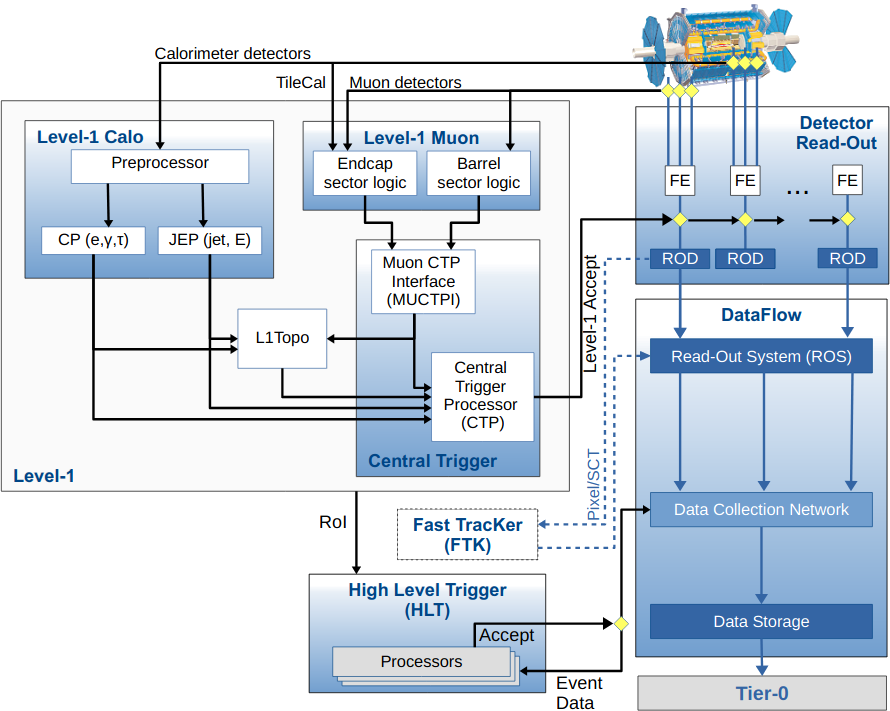
\includegraphics[scale=0.4]{ATLAS_Trigger_Flowchart}
			\caption{A figure showing the full ATLAS trigger chain from hits in the calorimeters and MS to delivery to CERN's Tier-0 computing infrastructure \cite{ATLASTrigger}.}
			\label{Fig:ATLASTriggerChain}
		\end{figure}
		
		\subparagraph{The L1Calo trigger} takes analogue input signals from the calorimeter, which are converted to digital signals and calibrated by the preprocessor. These digital signals are sent in parallel to the Cluster Processor (CP) and Jet/Energy-sum Processor (JEP) which identify object candidates and perform preliminary measurements. The CP identifies electron, photon, and $\tau$-lepton candidates, and the JEP identifies jet candidates and sums both the total and missing transverse energies. \par

		\subparagraph{The L1Muon trigger} analyses hits from the RPCs and TGCs of the MS to understand how the detected track pattern deviates from the hit pattern of a muon of infinite momentum.  The L1Muon trigger also applies a coincidence requirement on the outer TGCs, inner TGCs, and tile calorimeter in order to reduce the event rate from events occurring outside the IP. \par

		Information from the L1Calo Trigger, L1 topological (L1Topo) trigger, and L1Muon trigger passed through the L1Muon Central Trigger Processor Interface (MUCTPI) feed into the CTP where events are selected based on event-level quantities (e.g. total calorimeter energy), multiplicity of objects above thresholds (e.g. muon p$_{T}$), or topological requirements (e.g. invariant masses or angular distances) \cite{ATLASTrigger}. 
		
		The latency of the L1 trigger system is $< 2.5$ $\mu$s, which equates to making the full the decision to filter the event in under 2.5 $\mu$s of the bunch crossing occurring. This speed is possible by only performing initial triggering with the L1 trigger before passing events two the second stage of the ATLAS trigger system, the High Level Trigger (HLT). The L1 trigger reduces the LHC's full event rate of 40 MHz to a much more manageable size of 100 kHz. \par
		
		Events from the L1 trigger are sent to ReadOut Drivers (RODs) that process and format the data, then to the ReadOut System (ROS) which buffers the data in preparation for the HLT. This data contains the event information from the L1 trigger in addition to Regions-of-Interest (ROIs) in $\eta$ and $\phi$ marked by the L1 trigger, which are areas designated to be investigated by the HLT. 
		Unlike the hardware based L1 trigger, the HLT is entirely software base trigger requiring the collaboration of a server farm of approximately 40,000 processing units (PUs). \par 
		
		Standard event reconstruction begins with a series of dedicated fast trigger algorithms that aim to quickly reject events, before the surviving events undergo far more CPU-intensive algorithms for final event selection. Information from the ROS is only supplied to the HLT on request, as the more intensive reconstruction cannot keep pace with the speed of the L1 trigger. Typical reconstructions will often execute at least one feature-extraction algorithm that requests fragments of event data from within the RoIs supplied by the L1 trigger, and use the reconstructed features to decide if the specified trigger condition has been satisfied. Some cases require event information from the full detector, such as in the case of reconstructing missing transverse momentum which requires the reconstruction of all present physics objects. \par

		This rapid event reconstruction and analysis using the full detector granularity takes place with a latency of approximately half a second which, while far slower than the extremely high speeds of the LHC beamline and L1 trigger, is relatively quick when compared with day to day speeds. The HLT reduces the event rate from the 100 kHz input by the L1 trigger even further, to an average of 1 kHz \cite{ATLASTrigger2010}. Using the previous figure of 1.5 MB per event, this equates to a much more manageable data writing speed of 1.5 GB per second. Events passing the ATLAS trigger system are subsequently sent to CERN's Tier-0 computing infrastructure for full reconstruction. 

		% 11/02/21

		\newpage
		
		\bibliographystyle{Thesis.bst}
		
		\bibliography{Prog_2}	
				
\end{document}